 \documentclass[11pt,spanish]{report}
%\usepackage[square]{natbib}
\usepackage[spanish,activeacute,mexico]{babel}
\usepackage{listings}
\usepackage{color}
\addto\captionsspanish{
  \renewcommand{\contentsname}%
    {Tabla de Contenido}%
}



\usepackage[utf8]{inputenc}
\usepackage{TemplateFiles/UNAMThesis}
\usepackage{amsmath}
%\usepackage{amsfonts}
\usepackage{amssymb}
\usepackage{amsthm}
\usepackage{enumerate}
\usepackage{multicol}

\graphicspath{ {img/} }
\usepackage[Glenn]{fncychap}
%\usepackage[Rejne]{fncychap}
\usepackage{fancyhdr}
\usepackage{fancyvrb}
\usepackage[caption=false]{subfig}
\usepackage[width=16.5cm,top=2.5cm,bottom=2.5cm,headsep=1cm,bindingoffset=6mm]{geometry}
\usepackage{alltt}
\usepackage{hyperref}
\pagestyle{plain}

\logounam{escudo_UNAM}
%\logounam{Escudo-UNAM}
%\logoinstitute{Escudo-IBT}
\pagenumbering{roman}
\flushbottom

\theoremstyle{definition}

%\newtheorem{theorem}{Theorem}
%\newtheorem{acknowledgement}[theorem]{Acknowledgement}
%\newtheorem{algorithm}[theorem]{Algorithm}
%\newtheorem{axiom}[theorem]{Axiom}
%\newtheorem{case}[theorem]{Case}
%\newtheorem{claim}[theorem]{Claim}
%\newtheorem{conclusion}[theorem]{Conclusion}
%\newtheorem{condition}[theorem]{Condition}
%\newtheorem{conjecture}[theorem]{Conjecture}
%\newtheorem{corollary}[theorem]{Corollary}
%\newtheorem{criterion}[theorem]{Criterion}
%\newtheorem{example}{Ejemplo}
%\newtheorem{definition}{Definición}
%\newtheorem{exercise}[theorem]{Exercise}
%\newtheorem{lemma}[theorem]{Lemma}
%\newtheorem{notation}[theorem]{Notation}
%\newtheorem{problem}[theorem]{Problem}
%\newtheorem{proposition}[theorem]{Proposition}
%\newtheorem{remark}[theorem]{Remark}
%\newtheorem{solution}[theorem]{Solution}
%\newtheorem{summary}[theorem]{Summary}
%\newenvironment{proof}[1][Proof]{\textbf{#1.} }{\ \rule{0.5em}{0.5em}}


\begin{document}

\title{ Detección y Reconocimiento de objetos utilizando técnicas de visión en GPU }
\author{Jaime Alan Márquez Montes}

\institute{Posgrado en Ciencia e Ingeniería de la Computación}
\department{Laboratorio de Bio-Robótica}
\degree{Maestro en Ciencias de la Computación}

\supervisor{Dr. Jesús Savage Carmona \\ Dr. Jose David Flores Peñaloza }

\city{Ciudad de México, D. F.}
\degreemonth{Junio}
\degreeyear{2015}

\pdfbookmark[0]{Portada}{portada}
\maketitle

\begin{dedication}
Dedicatorias...........
			\\...........
			\\............
\end{dedication}

\begin{acknowledgements}
Agradecimientos...........
			\\...........
			\\............
\end{acknowledgements}

\pdfbookmark[0]{\contentsname}{toc}
\tableofcontents

\clearpage

%\begin{foreword}
%Redacte aqu\'{\i} el pr\'{o}logo contando la historia detr\'{a}s de su
%trabajo.
%\end{foreword}


\pagestyle{fancy}
\renewcommand{\chaptermark}[1]{\markboth{}{}}
\pagenumbering{arabic}

\chapter{Introducción}
\spacing{1.5}
\section{Contexto}
El software de los robots móviles en ocasiones es más complejo que el hardware que lo conforma. La complejidad del software dependerá  de cuánta interacción tenga el robot con su entorno. Una  parte esencial del software es la forma de interpretar y darle significado a los datos obtenidos de los diferentes sensores del robot. \\
La vista es a lo que más recurre un ser humano para obtener información de su entorno. Por ello no es de extrañarse que la visión computacional tenga una participación muy importante en la robótica, porque estas máquinas empiezan a ser utilizadas para tareas que antes solo los humanos realizaban, mismas que deben realizar de una manera adecuada y en tiempo.\\
El tiempo en el que se realizan las actividades en cualquier ámbito siempre ha sido importante. El paralelismo es la forma por la cual optaron los nuevos procesadores para mejorar su velocidad, ya que solo incrementar el número de pulsos de reloj por segundo implica problemas como la disipación de calor. Pero no todo es procesadores multinúcleo, las unidades de procesamiento gráfico por sus siglas en ingles GPU se pueden programar para realizar tareas de propósito general.\\

\section{Problema a resolver}
Los algoritmos que se utilizan en visión computacional aunque confiables consumen mucho tiempo de procesador, por lo cual se ha tratado de hacer más eficientes estos algoritmos, pero provocando que  la confiabilidad disminuya. El tiempo en el cual se adquiere y procesa la información es crucial en la actividad de un robot, pues de esto depende que decisión tomara.\\
Con base en lo anterior, tan importante es el tiempo en que procesemos los datos, para tomar una decisión, como importante es que la información obtenida sea congruente. En muchos casos, el software que se ejecuta en paralelo es más rápido que el secuencial. Los algoritmos que se manejan en visión computacional son  casi siempre secuenciales. Otro punto importante es que recursos como el procesador y la memoria de la computadora del robot siempre estarán siendo demandados por otros módulos del robot.\\

\section{Hipótesis} 
La finalidad del presente documento es  confirmar la siguiente hipótesis:
\begin{center}
\textit{"Por medio del uso de unidades de procesamiento gráfico de propósito general tener un mejor desempeño en la ejecución del algoritmo SIFT paralelo, comparado con una implementación secuencial del mismo"}
\end{center}
Respecto al alcance, se considerara valida la hipótesis si se pueden obtener los puntos característicos de una imagen con los cuales se podrían encontrar descriptores para su comparación. El desempeño se mide comparando el tiempo de ejecución entre el sistema actual del robot y el propuesto.\\

\section{Estructura de la tesis}
En el capítulo Marco Teórico se consideran dos puntos importantes que son la extracción y descripción de las características de una imagen. Aunado a esto  se explica el proceso para extraer puntos característicos y obtener el descriptor de cada uno de estos de una manera que sean tolerantes a diferentes transformaciones por medio del algoritmo de SIFT, y como es que han venido cambiado los procesadores hasta poder llegar a el computo en las GPU.\\
El capítulo Unidad de Procesamiento de Gráficos de Propósito General  se enfoca en cómo han cambiado los procesadores multinúcleo, la forma en la que los programamos y sobre todo el cómputo en cooperación con las tarjetas gráficas. Se enfoca en las GPU de la familia de nVidia, se comenta un poco de la historia de estos multiprocesadores, su arquitectura y el modo en que podemos programar estos dispositivos, que ya no son solo utilizados en gráficos.\\
En el Capítulo SIFT en GPU se presentan puntos importantes al momento de paralelizar un algoritmo: Cómo es que se propone dividir el algoritmo de SIFT para que sea más sencillo el proceso de paralelización, y como trabajan los kernels en general para este caso. Más adelante se explica cómo es que están estructuradas una a una las secciones, en las que dividimos el algoritmo.\\
Para el capítulo Pruebas y Resultados se compara el tiempo que toma obtener los puntos característicos SIFT con el sistema propuesto y algunos otros ya implementados como la librería OpenSIFT y OpenCV.\\
El capítulo Conclusiones y Trabajo a Futuro se tomaran en cuenta cuales fueron las ventajas y desventajas de haber paralelizado el algoritmo SIFT respecto a los resultados. Como es que benefician estos resultados y cuáles serían los puntos con los que se podría seguir adelante con este trabajo de investigación.  \\







\pagebreak

\chapter{Scale-Invariant Feature Transform SIFT}
	El algoritmo de SIFT, propuesto por Lowe en \cite{Lowe2004},  provee un método robusto para la extracción de puntos característicos que se utilizan para generar el descriptor. Los puntos que se encuentran son invariantes a diferentes transformaciones como traslación, escalamiento y rotación. Han mostrado tener un amplio rango de tolerancia a transformaciones afines, adición de ruido y cambios de iluminación. A continuación se describirán los pasos del algoritmo para la generación del conjunto de puntos característicos:

	\section{Detección de puntos extremos en el Espacio-Escala} \hfill \\
		Se realiza una búsqueda en las imágenes en todo el espacio escala, para localizar puntos extremos se debe identificar su ubicación y escala, para volver a encontrarlos no importando la vista o tamaño del mismo objeto.\\
		El espacio escala es un conjunto de imágenes, que se forman a partir de suavizar la imagen original a diferentes niveles de detalles, los cuales son definidos por un parámetro $\sigma$. Está representado por la función $L(x,y;\sigma)$ la cual se forma por la convolución con $G(x,y;\sigma)$ y la imagen original $I(x,y)$:
		$$L(x,y;\sigma) = G(x,y;\sigma) * I(x,y)$$
		Donde $*$ es el operador convolución en $x$ y $y$, y
		$$ G(x,y;\sigma) = \frac{1}{2\pi\sigma^2}e^{\frac{-(x^2+y^2)}{2\sigma^2}}$$
		\begin{figure}[h]
			\centering
				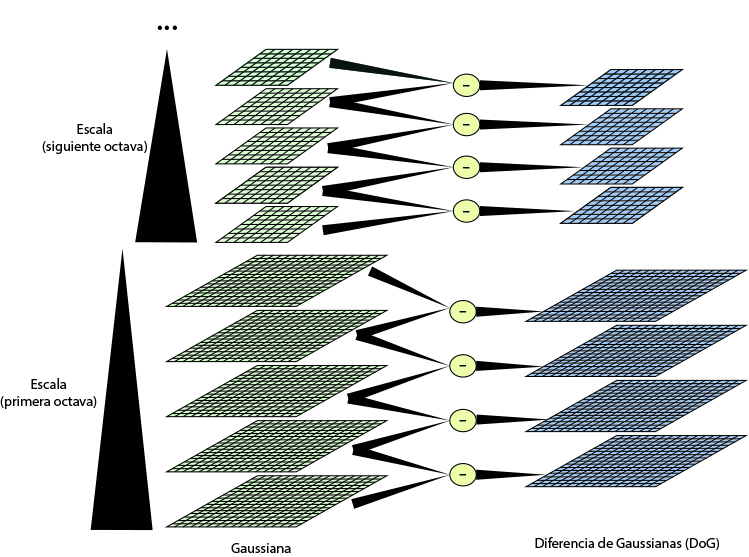
\includegraphics[scale=0.5]{img/spaceScale.jpg}
			\caption{Espacio Escala de Diferencia de Gaussianas}
		\end{figure}		
		Para la detección de puntos extremos estables se aplicará el espacio escala, usando diferencias de gaussianas convolucionadas con una imagen, en lugar de solo un filtro gaussiano, $D(x,y;\sigma)$  que podremos calcular por la diferencia de dos escalas cercanas separadas por un factor $k$ multiplicativo:
		$$D(x,y;\sigma) = (G(x,y;k\sigma) - G(x,y;\sigma)) * I(x,y)$$ $$= L(x,y;k\sigma) - L(x,y;\sigma)$$
		La diferencia de gaussianas es una aproximación muy cercana a el laplaciano de gaussiana (LoG) normalizado en escala, $\sigma^2 \nabla^2 G$. La normalización hecha con el factor $\sigma^2$ es necesaria para poder asegurar que el algoritmo sera invariante a los cambios en tamaño. La relación entre D y $\sigma^2 \nabla^2 G$ es una ecuación en derivadas parciales:
		$$\frac{\partial G}{\partial \sigma} = \sigma \nabla^2 G$$
		Podemos ver que $\nabla^2 G$ se puede calcular con una aproximación de diferencias finitas de  $\frac{\partial G}{\partial \sigma}$, usando diferencias de escalas próximas de $k\sigma$ y $\sigma$:
		$$ \sigma \nabla^2 G = \frac{ \partial G}{\partial \sigma} \approx  \frac{G(x , y , k \sigma) - G( x , y, k \sigma)}{k \sigma - \sigma}$$
		y por lo tanto,
		$$ G(x , y , k \sigma) - G( x , y, k \sigma) \approx (k - 1)\sigma^2 \nabla^2 G $$
		En la figura 3-1 se puede ver la construcción de $D(x,y,\sigma)$. La imagen inicial se convoluciona con diferentes mascaras gaussianas, para producir imágenes separadas por un factor constante $k$ en el espacio escala. Se divide cada octava del espacio escala entre un numero entero, s, de intervalos entonces $k= 2^\frac{1}{s}$. Se producen $s+3$  imágenes emborronadas en la pila, por octava.
		\begin{figure}[h]
			\centering
				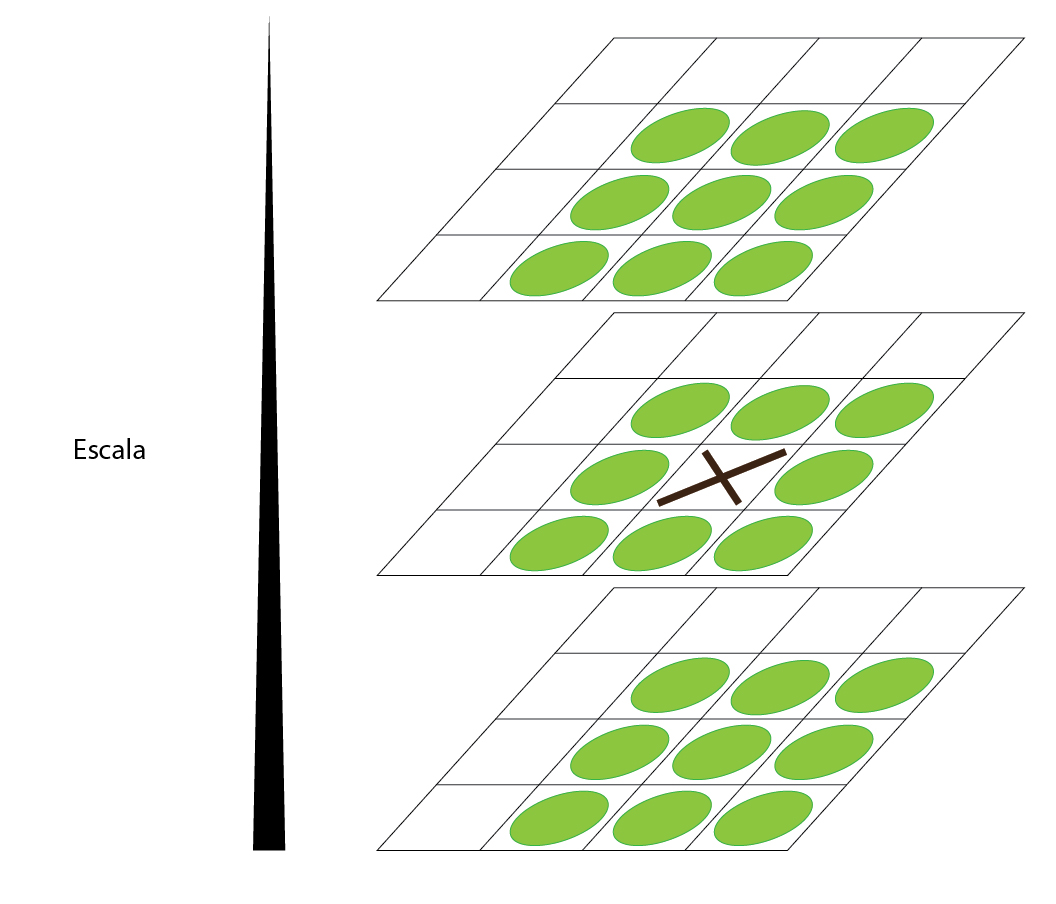
\includegraphics[scale=0.3]{img/EscalaPuntosExtremos.jpg}
			\caption{Espacio Escala de Diferencia de Gaussianas}
		\end{figure}
		Para extraer las ubicaciones máximas y mínimas (puntos extremos) en $D(x,y,\sigma)$, cada punto es comparado con sus ocho vecinos en la misma imagen y con sus otros dieciocho vecinos de escala, nueve en la imagen de arriba y nueve en la imagen de abajo (Figura 3-2). Solo se selecciona el punto si es el más grande o el más pequeño de entre todos sus vecinos.
	
	

	
	\section{Localización de puntos característicos} \hfill \\ 
		Una vez que se seleccionaron los puntos extremos, se aplica una medida de estabilidad sobre todos para descartar aquellos que no sean adecuados, para obtener puntos  característicos de forma precisa. Existen dos casos donde los puntos extremos anteriormente seleccionados tendrían que ser eliminados:
	\begin{enumerate}
		\item El punto tiene un contraste muy bajo.
		\item El punto está localizado sobre un borde.
	\end{enumerate}			
	Para eliminar los puntos del caso uno, primero debemos obtener la serie de Taylor del espacio escala $D(x,y,\sigma)$:
		$$D(X)=D +\frac{\partial D}{\partial X}^T X+ \frac{1}{2} X^T\frac{\partial^2 D}{\partial X^2} X $$
		donde la $D$ y su derivada son evaluadas en el punto $X = (x,y,\sigma)^T$ cuando se deriva esta función respecto a $X$ y se iguala a cero podemos encontrar los valores extremos: 
	    $$ \hat{X} = - \frac{\partial^2 D}{\partial X^2}^{-1}\frac{\partial D}{\partial X}$$
	 	La función que evaluara al punto extremo sera, $D(\hat{X})$, la cual rechazara al punto si es de muy bajo contraste, la cual se obtiene de sustituir $\hat{X}$ en $D(X)$:
	 	$$D(\hat{X})=D + \frac{1}{2} \frac{\partial D}{\partial X}^T \hat{X} $$ 	 
	 	En el trabajo de Lowe \cite{Lowe2004}, se  puede ver que encontraron experimentalmente que cualquier valor extremo menor de 0.03 es descartado:
	 	$$ |D(\hat{X})|< 0.03$$ 	 
	 	Para el segundo caso, se utiliza una matriz Hessiana de $2\times2$, $H$, la cual se calcula en la escala y lugar del punto extremo:
		$$ 
		H
		=
		\begin{bmatrix}
			D_{xx} & D_{xy}\\
    		D_{xy} & D_{yy}
		\end{bmatrix}		 	
		$$	
		Los valores propios de H son proporcionales a las curvaturas de D. Se toma prestado el criterio que se usa para la detección de esquinas usando el algoritmo de Harris \cite{Harris1988}, se puede evitar el calculo de los valores propios ya que solo nos interesa su relación. Sea $\alpha$ el valor propio de mayor magnitud y $\beta$ el de menor. Entonces podemos calcular la suma de los valores propios de la diagonal de $H$ y su producto por medio del determinante:
		$$Tr(H) = D_{xx} + D_{yy} = \alpha+\beta,$$ $$Det(H) = D_{xx}D_{yy}-(D_{xy})^2= \alpha\beta$$
		Sea $r$ la razón de la magnitud que existe entre $\alpha$ y $\beta$, $\alpha = r\beta$. Entonces:
		$$\frac{Tr(H)^2}{Det(H)}= \frac{(\alpha+\beta)^2}{\alpha\beta}= \frac{(r\beta+\beta)^2}{r\beta^2}= \frac{(r+1)^2}{r}$$
		el cual solo depende de la razón de los valores propios y no de los valores individuales. El valor de $\frac{(r+1)^2}{r}$, es mas pequeño cuando los valores propios son iguales e incrementa con $r$.Entonces para cerciorar que la razón de las curvas principales es menor que cierto umbral, $r$, solo se necesita:
		$$\frac{Tr(H)^2}{Det(H)} < \frac{(r+1)^2}{r}$$
		En la publicación de Lowe \cite{Lowe2004} se encontró un valor experimental para $r=10$, que elimina los puntos extremos que tengan la razón entre las dos curvas mayor que 10.
	
	
	\section{Asignación de orientación} \hfill \\
		Por medio de la asignación de una orientación a cada punto característico, basado en propiedades locales de la imagen, el descriptor que encontremos sera invariante a la rotación. La ubicación en el espacio escala del punto característico, es usada para seleccionar la imagen suavizada por una mascara gaussiana, $L$, esto provocara que sea invariante a la escala. Para cada muestra de la imagen, $L(x,y)$, la magnitud del gradiente, $m(x,y)$, y la orientación ,$\theta(x,y)$, son precalculadas por medio de diferencias de gaussianas:
  		$$m(x,y) = \sqrt{ (L(x+1,y)-L(x-1,y))^2 + (L(x,y+1)-L(x,y-1))^2 }$$		
		$$\theta(x,y) =  \tan^{-1} \left(\frac{L(x,y+1)-L(x,y-1)}{L(x+1,y)-L(x-1,y)}\right)$$
		Se formara un histograma de orientaciones que tendrá la orientación de los gradientes calculados en una región, al rededor del punto característico, el tamaño de esta muestra dependerá de la ubicación en el espacio escala en la que se encuentre el punto característico. El histograma de orientaciones tendrá 36 divisiones cubriendo los 360 grados.
		
		
		\begin{figure}[h]
			\centering
				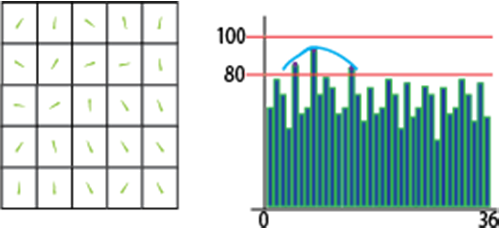
\includegraphics[scale=0.7]{img/HistoOrientacion.png}
			\caption{Histograma de Orientación }
	\end{figure}
		
		Para cada muestra agregada se ponderada por la magnitud de su gradiente y por una mascara circular gaussiana ponderada con $\sigma$, que es $1.5$ veces que de la ubicación del espacio escala donde reside el punto característico.\\
		\pagebreak
		Los picos en el histograma de orientación corresponden a las direcciones dominantes de los gradientes locales. Se encuentra el pico mas grande y cualquier otro pico que se encuentre en el rango de $100\% - 80\%$, del pico más grande, se utiliza para hacer que el punto característico tenga una orientación. Para ubicaciones con varios picos de magnitudes similares, se generaran puntos característicos con la misma ubicación y escala pero con diferentes orientaciones. Solo el $15\%$ de los puntos se les asignan múltiples orientaciones, pero aun así esto contribuye mucho al momento de emparejar. Finalmente se obtiene una parábola usando como puntos tres picos cercanos entre si, para interpolar la posición del pico con mas precisión.  \\\\\\\\\\\ \pagebreak
	
	
	

		

\section{Descriptor de puntos característicos} \hfill \\

		
	Hasta este momento tenemos una colección de puntos característicos, los cuales están formados por una ubicación, una escala y una orientación. Ahora debemos formar un descriptor que sea lo suficientemente distintivo. Para esto tenemos que tomar una muestra de la imagen, al rededor del punto característico de $16\times16$ pixeles y se dividirá en una región de $4 \times 4$. Se generará un histograma de orientación de los gradientes de cada región, a diferencia del histograma de orientación explicado anteriormente, el histograma solo tiene 8 divisiones con las cuales se cubrirán los 360 grados, igualmente se usara una ponderación gaussiana para la asignación de la magnitud al histograma.
		
	Al final el descriptor de cada punto característico estará formado por un vector, que tiene las ocho orientaciones de los $4\times4$ histogramas. Por lo tanto el tamaño del vector sera de $4\times4\times8 = 128$ elementos. 
 	
	\begin{figure}[h]
			\centering
				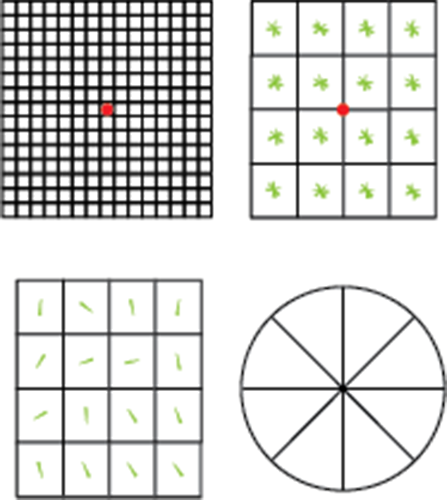
\includegraphics[scale=0.5]{img/Descriptor.png}
			\caption{Descriptor }
	\end{figure}
		
 
 








\pagebreak
\chapter{Computo en GPU's}
Hasta hace 12 años la velocidad a la que crecían cada generación de procesadores era increíble, los programas eran tan rápidos como cada nueva generación de procesadores. Este crecimiento entre cada generación se detuvo, el problema es el consumo de energía y la disipación de calor, no permiten aumentar la frecuencia del reloj del procesador y el nivel de actividades por ciclo, en una sola unidad de procesamiento (CPU). Todos los productores de procesadores migraron a un nuevo modelo, los procesadores multinúcleo incrementaron el poder de procesamiento.

Este cambio en los procesadores tuvo un gran impacto a los programadores, la mayoría de las aplicaciones son escritas de forma secuencial,  por que la ejecución de estas son comprensibles paso a paso, mediante el código. Pero un programa secuencial ejecutándose en un solo núcleo del procesador, no sera más rápido. Entonces los programadores ya no pueden agregar cualidades y capacidades a sus programas.

Llega el momento de cambiar, si se desea que la calidad de los programas siga escalando con cada generación de procesadores, se deben crear programas que trabajen con múltiples hilos, cooperando todos para completar un trabajo mas rápido. Existen dos corrientes principales en cuanto a los procesadores multi-núcleo, el primero, es donde se pretende mantener la velocidad de los programas secuenciales, mientras se mueven entre múltiples núcleos; la segunda, se centra mas en la ejecución de aplicaciones en paralelo, tiene un gran numero de núcleos pequeños que va creciendo con cada generación. Es esta rama en la que entran las unidades de procesamiento gráfico o por sus siglas en ingles GPU.\cite{Kirk2010}

\section{GP-GPUs Nvidia}

"Las GPU han evolucionado al punto que muchas aplicaciones del mundo real se están implementando fácilmente en ellas y se ejecutan muchísimo más rápido que en sistemas con múltiples núcleos. Las arquitecturas de computación del futuro serán sistemas híbridos con GPU de núcleos paralelos trabajando en tándem con CPU de múltiples núcleos".\cite{GPUIntro}

\begin{figure}[h]
			\centering
				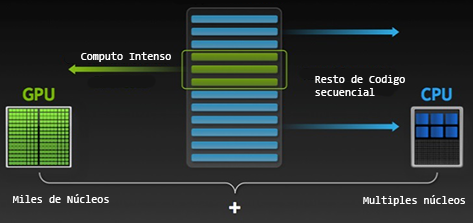
\includegraphics[scale=1]{img/how-gpu-acceleration-works.png}
			\caption{Sistema Híbrido}
\end{figure}

\subsection{Breve Historia}
La necesidad de mejores gráficos para los vídeo juegos, provocaron un gran avance en el hardware que se diseñaría. Desde principios de 1980 hasta finales de 1990 las tarjetas dedicadas a gráficos, no eran más que pipelines fijos que despliegan las formas geométricas calculadas por el CPU, por medio del hardware de acceso directo a memoria, por sus siglas en ingles DMA, esto les daba un funcionamiento fijo y apenas se podía configurar, con principalmente dos API, OpenGL de \textit{Silicon Graphics} y Direct3D de \textit{Microsoft}. Un ejemplo de estas tarjetas gráficas es, a la que se le acuño el nombre de GPU, la GeForce 256\cite{GeForce256} lanzada al mercado en 1999, aporta una capacidad visual sin precedentes, capaz de realizar las funciones de  transformación, iluminación, organización y rendering, con la capacidad de procesar 15 millones de triángulos por segundo y un rendimiento de 480 millones de píxeles por segundo. Su motor de rendering  256 bits muestra una mejora en cuanto a la complejidad visual.

Toda esta tecnología tan revolucionaria llamo la atención de otros profesionales, que se integraron a el trabajo de los artistas y desarrolladores de vídeo juegos, utilizando el gran rendimiento de punto flotante que tenían los GPU para otros objetivos. De esta forma surge el movimiento de la GPU para fines generales(GP-GPU).

Pero en ese momento, la GP-GPU era muy difícil de manipular, solo aquellos que tenían amplios conocimientos en lenguajes de programación de gráficos, desarrollaban para esta plataforma. Pero aun que memorizaras el API entera se enfrentaba un reto, donde los cálculos para resolver problemas generales debían ser representados por triángulos o polígonos.

Fue hasta 2001, en la Universidad de Stanford un equipo, liderado por Ian Buck, que se propuso ver el GPU como un  \textit{procesador de flujos}. Este equipo desarrollaría \textit{Brook} \cite{Buck2001}, un lenguaje de programación diseñado para ser igual a la sintaxis de C, con algunas características adicionales. El lenguaje se desarrolla con el objetivo de minimizar el complejo trabajo de análisis, que se requería para generar aplicaciones paralelas. Introducirían conceptos como los flujos(streams), kernels y los operadores de reducción. Todo esto le dio un gran impulso a los GPU como procesadores de propósitos generales, ya que el lenguaje era mas fácil de manejar, ya que era de más alto nivel, y lo mas importante los programas escritos en \textit{Brook} eran hasta 7 veces mas rápido que códigos similares existentes.

La compañía NVIDIA se dio cuenta que tenia un hardware muy poderoso en las manos, pero debía complementarlo con herramientas de hardware y software intuitivas, con ello le hicieron la invitación a Ian Buck para colaborar con ellos, el objetivo sería ejecutar C a la perfección en una GPU. NVIDIA alcanza este objetivo en 2006 con el lanzamiento de CUDA, la cual seria la primera solución para las GP-GPU, y aunado a esta solución, lanza la GeForce 8800 la cual fue diseñada, para ser usada en cómputo de propósito general, y su arquitectura fue pensada en la de CUDA. 

\section{CUDA}
Compute Unified Device Architecture (CUDA) es una plataforma para computo paralelo y un modelo de programación, que NVIDIA lanzo en noviembre de 2006, permitiendo obtener aumentos en los rendimientos del computo, esto es gracias a la ayuda que la unidad de procesamiento de gráficos, le proporciona al CPU. 

Los dispositivos CUDA aceleran la ejecución de los programas que tienen una gran cantidad de datos a procesar, ya que la arquitectura de esta plataforma, de la cual se hablara adelante, es como un procesador tradicional como el que las computadoras tienen, solo que tienen la cualidad de que los procesadores son masivamente paralelos equipados con una gran cantidad de unidades aritméticas. En las cuales se ejecutara la misma instrucción en todas, respecto a la taxonomía de Flynn, la categoría seria de \textit{una instrucción, multiples datos} (SIMD). 

\begin{figure}[h]
			\centering
				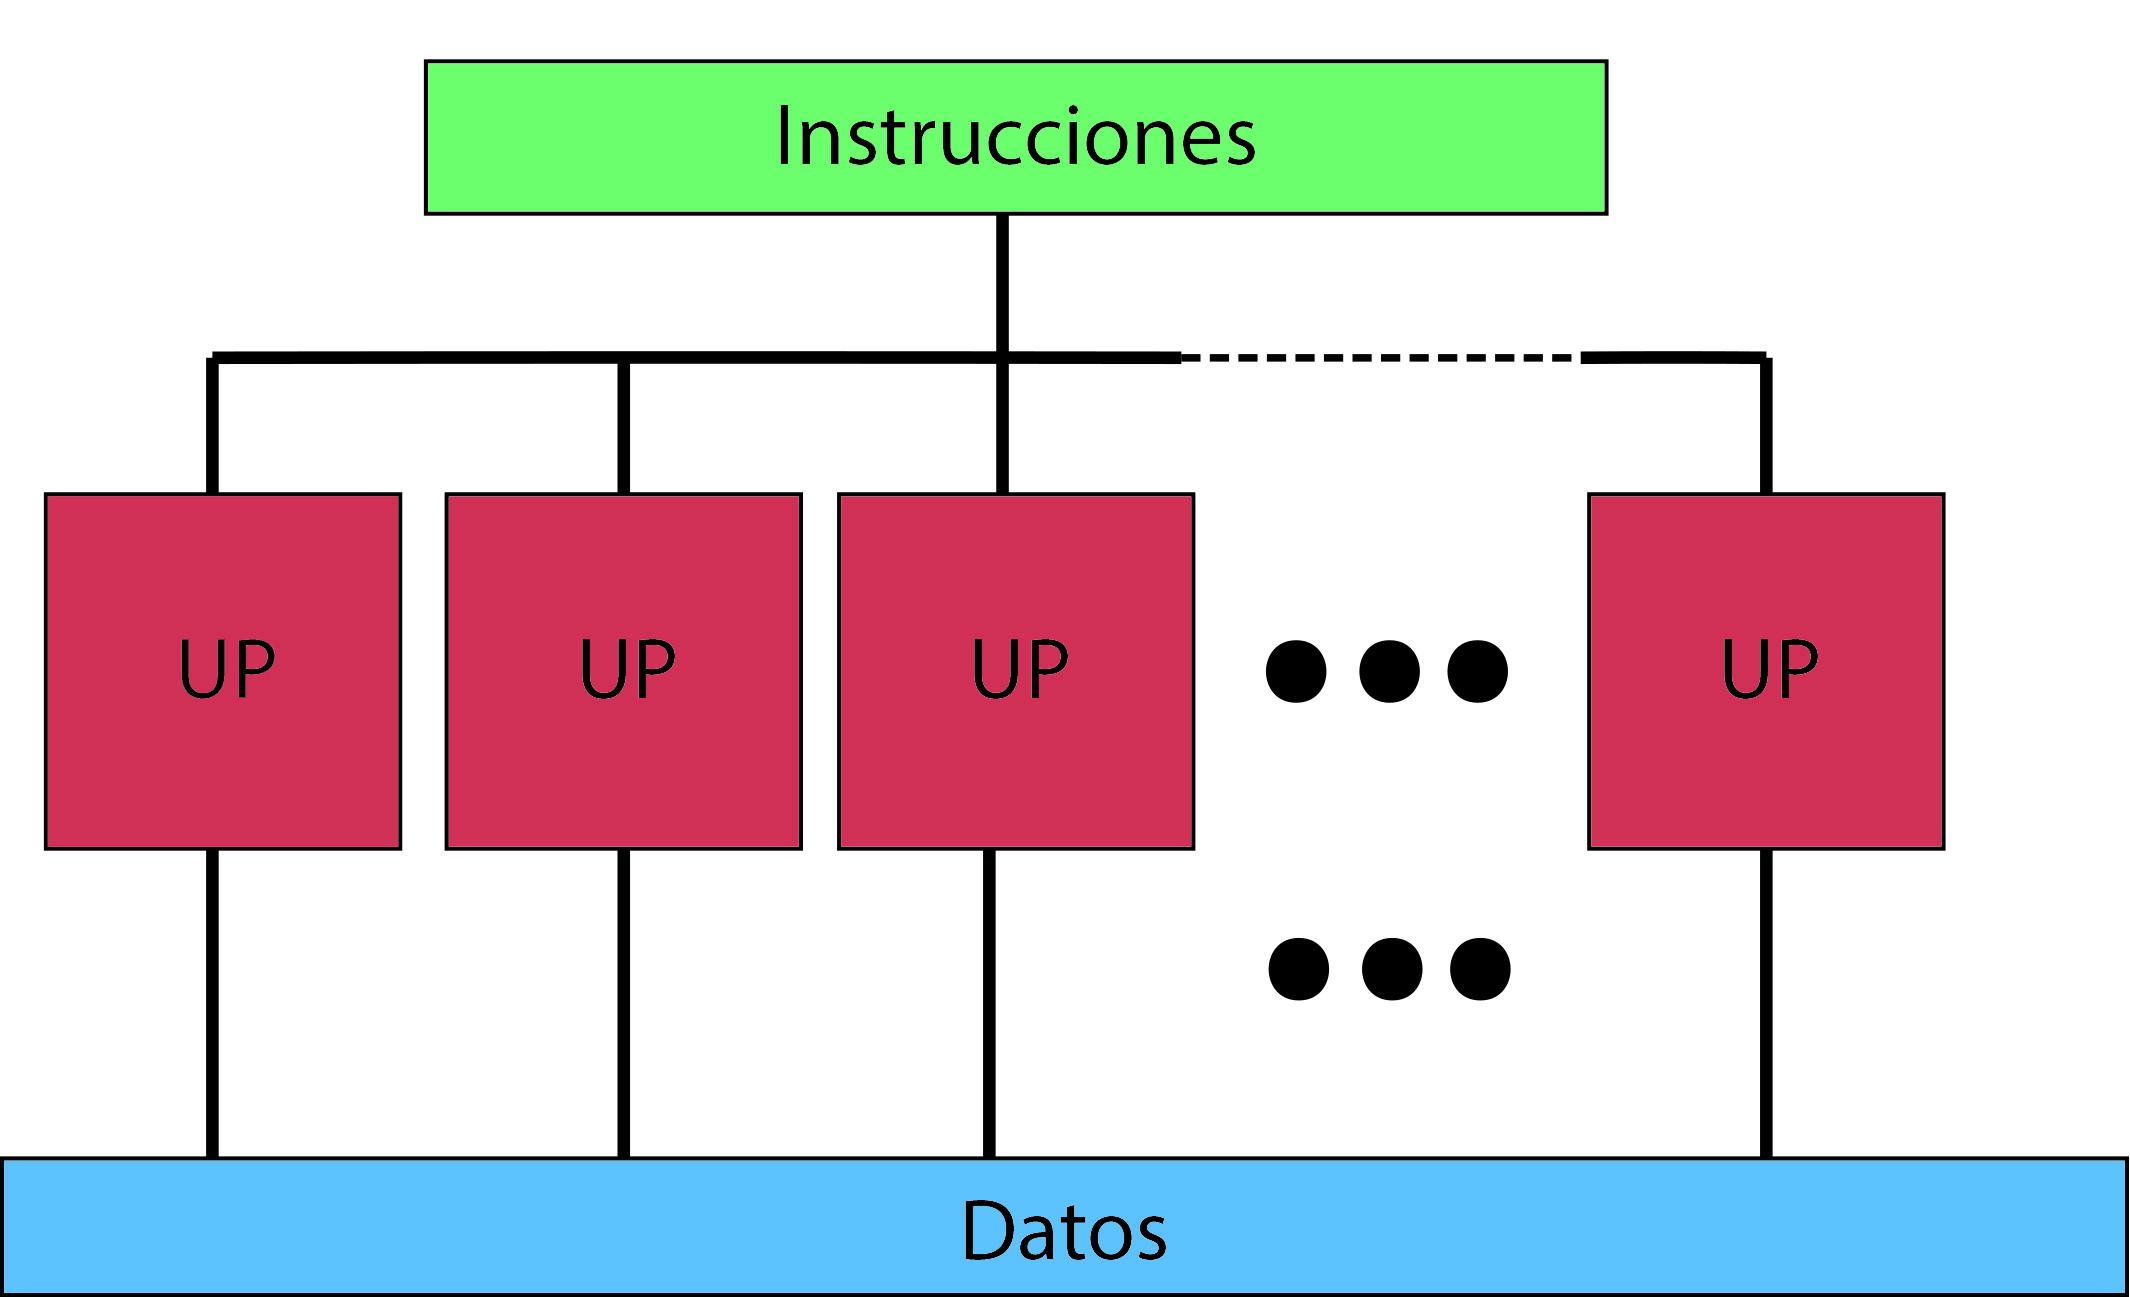
\includegraphics[scale=0.1]{img/SIMD.jpg}
			\caption{SIMD}
\end{figure}


Respecto al modelo de programación para desarrollar los programas para las GPU, es gracias a una extensión del lenguaje C, conocida como CUDA C. Existen alternativas a esta extensión, se pueden utilizar lenguajes como FORTRAN, Python, .NET combinando CUDA con Microsoft's F\# o alguna API como OpenCL u OpenACC\cite{lenguajes}. 
 

\subsection{Arquitecturas}
La arquitectura de CUDA fue diseñada, para que la GPU pudiera ser utilizada en aplicaciones de propósito general. En la cual se tiene un arreglo de procesadores con múltiples unidades aritmético lógica, por sus siglas en ingles ALU, las cuales para alcanzar este objetivo, fueron diseñadas para poder realizar operaciones de punto flotante, cumpliendo los requisitos del Instituto de Ingeniería Eléctrica y Electrónica (IEEE). Aparte de esto las ALU debían tener acceso a diferentes tipos de memoria, como la compartida entre unidades y la memoria de la tarjeta gráfica. 

Estas ALU tan particulares, en la arquitectura de CUDA las conoceremos como \textit{CUDA cores}, conforman gran parte de los Streaming Multiprocessor (SM). Los SM son procesadores que tienen la tarea de ejecutar los hilos concurrentemente, aparte de los CUDA cores tienen, están formados por una memoria cache(shared memory), registros y algunas unidades de funciones especiales.

\subsubsection{Fermi}

Los GPU basados en la arquitectura Fermi \cite{fermi}, están formados por 512 CUDA cores. Los CUDA cores ejecutan operaciones de punto flotantes o enteras por ciclo de reloj, y por cada uno de los hilos. Los 512 CUDA cores están organizados en 16 SM de 32 cores cada uno. El GPU tiene seis particiones de memoria de 64-bits, capacidad para leer 384-bits de la memoria simultáneamente y con una capacidad de hasta 6GB de memoria DRAM categoría DDR5. El sistema de conexión entre el GPU y el CPU es vía PCI-Express. La forma en que se hace la programación de el trabajo a realizar en cada bloque es asignado por un modulo llamado \textit{GigaThread}, este pasa las tareas a cada SM para que el haga la asignación de trabajo a cada hilo. 

\begin{figure}[h]
			\centering
				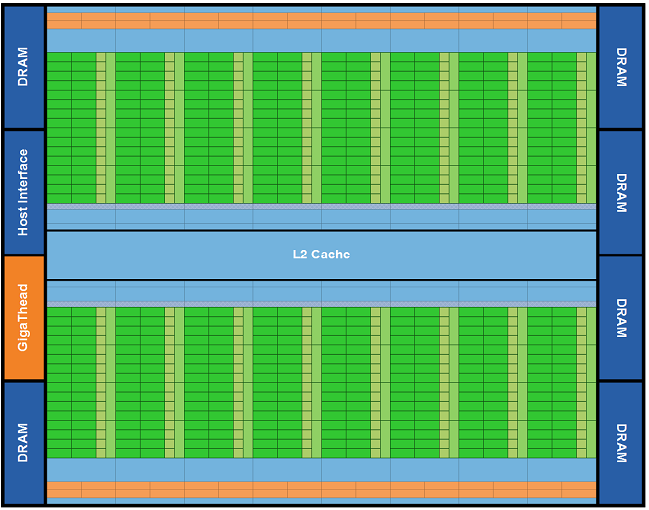
\includegraphics[scale=0.7]{img/ArqFermi.png}
			\caption{La arquitectura Fermi tiene sus 16 SM al rededor de la memoria compartida L2 cache}
\end{figure}

La arquitectura tuvo mejoras significativas como el rendimiento en las operaciones de doble precisión, dedicado a computo científico; soporte para la corrección de errores, para asegurar las operaciones con números muy grandes, en aplicaciones delicadas; se implemento una jerarquía en la memoria cache, que permite aumentar la eficiencia en cuanto a las  lecturas a memoria; la memoria compartida tuvo un incremento; y las operaciones atómicas incrementaron su desempeño, gracias a que se aumentaron las unidades de operaciones atómicas y la aparición de la memoria L2 cache. 

\begin{figure}[h]
			\centering
				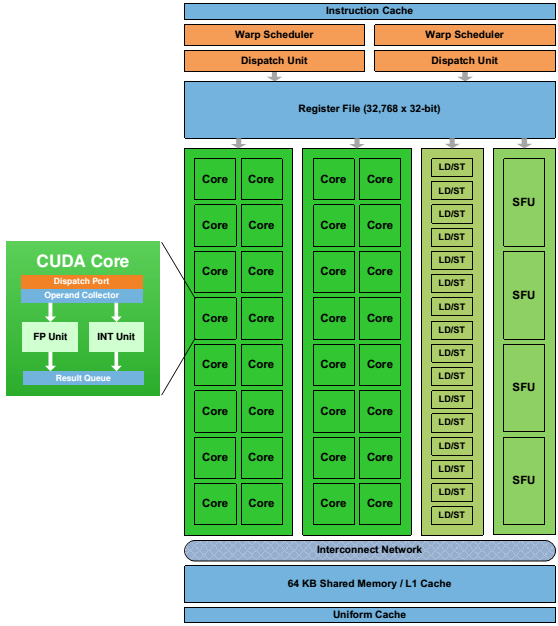
\includegraphics[scale=0.6]{img/fermiSM.png}
			\caption{Fermi Streaming Multiprocessor (SM)}
\end{figure}

Las SM de la arquitectura Fermi están formadas de diferentes elementos, iniciando por los 32 CUDA cores, cada uno con una unidad aritmética lógica para las operaciones con enteros y una unidad de punto flotante. Cumplen con la norma IEEE 754-2008 que permite realizar una multiplicación y una suma en un solo paso de redondeo. La asignación de trabajo en las SM se realiza por el modulo \textit{GigaThread}, que divide en bloques de hilos a cada SM, después los planeadores de \textit{warps} es quien tienen el trabajo de dividir este bloque en grupos de 32 hilos para su ejecución dentro de la SM. Tambien tiene 16 unidades load/store, las cuales permiten calcular origen y destino de dieciséis hilos por pulso de reloj; cuenta también con 4 unidades de funciones especiales (SFU), que ejecutan instrucciones mas complejas como senos, cosenos, reciproco y raíz cuadrada. 

\subsubsection{Kepler}

La arquitectura Kepler \cite{Kepler}, modifico los SM de su antecesor llamándolo Next Generation Streaming Multiprocessor (SMX), es el nuevo procesador de esta arquitectura, en la cual encontraremos que esta formada por 15 de estos procesadores y seis controladores de memoria de 64-bits.La cantidad de CUDA cores que contiene es de 192 de precisión simple y 64 unidades de doble precisión. 

Las unidades load/store aumentaron a 32 y las SFU también incrementaron a 32, ocho veces más que en Fermi. La asignación de hilos dentro de el SMX es programado igualmente por planeadores de warps, bloques de 32 hilos, Kepler tiene 4 planificadores de warps, de esta manera se tienen 2 unidades de despacho de instrucciones, permitiendo repartir y ejecutar 4 warps de manera concurrente. Nos encontramos con una memoria cache L1, la cual podemos cambiar su configuración. 

\begin{figure}[h]
			\centering
				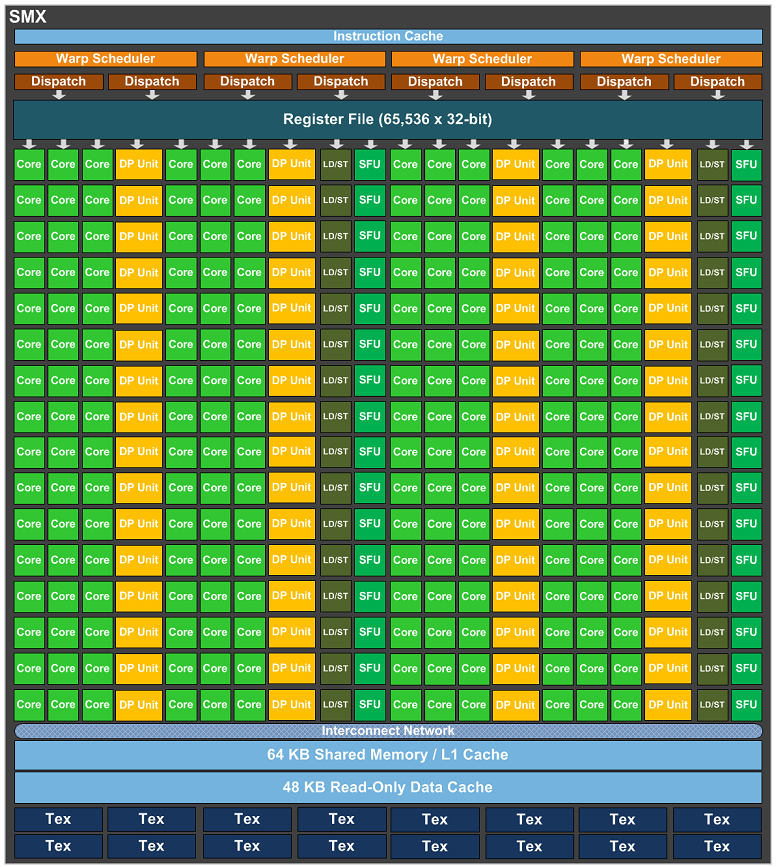
\includegraphics[scale=0.4]{img/KeplerSMX.png}
			\caption{Kepler Next Generation Streaming Multiprocessor (SMX)}
\end{figure}

La capacidad de esta memoria es de 64KB, se pueden tener las configuraciones de 16, 32 o 48 KB para la memoria cache, dejando el resto para la memoria compartida. La cantidad de registros por SMX es de 65536, de los cuales, cada hilo puede tener acceso a 255 registros para el almacenamiento de datos. La memoria de textura ha sido un recurso valioso para para programas donde se requiere probar o filtrar datos de una imagen, en esta arquitectura dejo de ser un hardware dedicado solo a este objetivo, se dejo un espacio en la memoria global de solo lectura de 48KB que funciona como una memoria cache para agilizar las lecturas.



En esta arquitectura se agrego una característica, donde no se requiere de el CPU para lanzar programas en la GPU, lo que significa que el GPU tiene la capacidad de generar mas carga de trabajo, administrar recursos y obtener resultados dentro de la misma GPU, en la zona de mas interés, donde se pueda requerir más poder de computo. 

\begin{figure}[h]
			\centering
				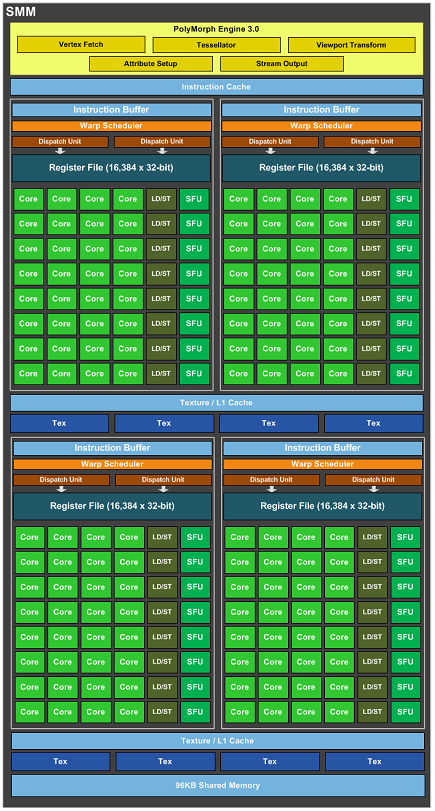
\includegraphics[scale=0.45]{img/MaxwellSM.png}
			\caption{Maxwell Streaming Multiprocessor (SMM)}
\end{figure}



\subsubsection{Maxwell}
La arquitectura Maxwell\cite{Maxwell}, tuvo un cambio en su diseño para proporcionar un cambio dramático en su desempeño. Lo que genero este desempeño fue el nuevo diseño que le dieron a los nuevos SM llamados SM Maxwell (SMM). El numero de CUDA cores bajo a 128, para poder separarlos en 4 divisiones de 32 CUDA cores, cada una de esas divisiones tiene un planificador de warps, para su bloque de 32 CUDA cores, el cual es capaz de despachar dos instrucciones por ciclo de reloj. Estas divisiones hicieron que se utilizara de una manera mas eficiente el espacio y la energia gastada para el manejo de la transferencia de datos.

La memoria compartida incremento a 96KB, la cual ya no se comparte con la memoria cache L1, ahora la memoria de textura comparte espacio con la cahce L1. Los registros, las SFU, y las unidades load/store siguen siendo la misma cantidad.



\subsection{Modelo de Programación}
\subsection{Rendimiento}


\pagebreak

\chapter{ SIFT en GPU}

La correcta paralelización de un algoritmo no es nada trivial. Después de el capitulo anterior, al ver todas las ventajas que tenemos en los GPU`s podríamos decir que son la solución a todo, tristemente no lo son, existen algoritmos que por la estructura del programa y forma de ejecutar el proceso, no se podrían paralelizar. Para saber como analizar si un algoritmo es paralelizable primero debemos dar una definición de que es un programa paralelo:

\begin{center}
\textit{"Programa paralelo es la especificación de dos o mas procesos simultáneos que cooperan entre si con un fin en común"}
\end{center}

Podemos sacar dos aspectos importantes de esta definición el primero es la comunicación, los procesos deben poder compartir información  para poder trabajar simultáneamente sobre un mismo problema; el segundo es la sincronización, es simplemente como organizar a los procesos para que mientras realizan su parte de trabajo sin que se interfieran entre ellos.
Entonces tenemos que cambiar la forma en que programamos, ahora no solo pensaremos como llegar a un objetivo paso a paso, sino  que debemos pensar como muchos procesos trabajaran juntos para alcanzar un objetivo, esto inmediatamente me da la idea de repartir o dividir el trabajo entre todos ellos. Así que para realizar la labor de paralelizar el algoritmo debemos analizar básicamente tres casos de paralelismo:
 
\begin{itemize}
 
	\item \textit{Funcional}: Aquí lo que se divide es el algoritmo, buscamos pasos en el algoritmo que no dependan de otra parte del mismo y los ponemos a ejecutarse simultáneamente en diferentes procesos. Requiere de sincronizan muy cuidadosamente para que las diferentes partes de el algoritmo no interfieran entre si. 
	
	\begin{figure}[h]
			\centering
				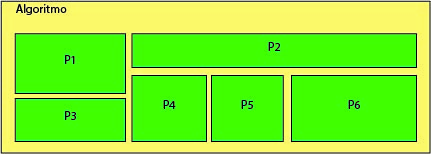
\includegraphics[scale=0.7]{img/funcional.jpg}
			\caption{Todos los procesos son partes diferentes del algoritmo}
	\end{figure}

	\item \textit{Dominio}: Se repartirán los datos en los múltiples procesos los cuales tienen una especificación idéntica. El sincronizan es sencillo en este caso, pero aun así hay que presentar atención ya que podríamos corromper información.
	\begin{figure}[h]
			\centering
				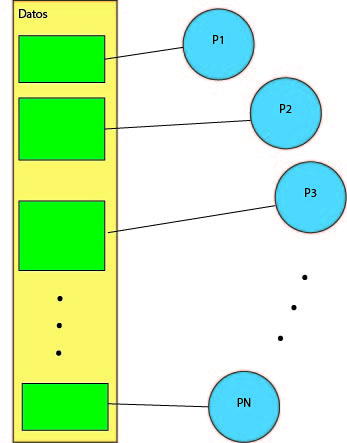
\includegraphics[scale=0.6]{img/dominio.jpg}
			\caption{Todos los procesos tienen la misma especificación }
	\end{figure}

	\item 	\textit{Actividad}: Es una combinación de los dos puntos anteriores.
\end{itemize}

Ahora que tenemos el algoritmo y las herramienta para mejorar su rendimiento por medio de la paraleización. Veremos como analizamos las partes de SIFT para de esta manera adaptarlo al modelo de programación de CUDA.
\pagebreak
\section{Análisis de SIFT para su Paralelización en GPU}

En esta sección se describe como se comunicaran y sincronizar los procesos, así como la estructura que tomara el algoritmo de SIFT, para poder paralelizarlo con CUDA. 

Primero dividiremos en 6 partes el algoritmo de SIFT, como se muestra en la figura 4-3 , estas partes no se ejecutaran simultáneamente, es solo que el algoritmo es bastante largo y al separarlo en estas partes podemos simplificarlo en diferentes kernels, que tendrán una secuencia de ejecución. 

\begin{figure}[h]
			\centering
				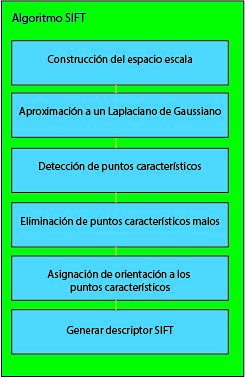
\includegraphics[scale=1]{img/SIFTdiv.jpg}
			\caption{División del algoritmo SIFT a paralelizar}
\end{figure}



Los kernels de las diferentes partes del algoritmo tienen una estructura en común, básicamente todos tiene como entrada una o mas imágenes, las cuales serán de solo lectura, y obtendremos una imagen o varias de salida. Cada proceso tendrá una sección de la imagen de tamaño  $N \times N$, la cual puede estar traslapada con la de algún otro proceso, pero esta área no requiere de sincronizar entre procesos ya que solo sera para obtener datos, para procesarlos.En la imagen de salida el proceso se le sera asignado solo un pixel de la imagen para escribir, como se puede mostrar en la figura 4-4 las zonas del P1 y P2 están traslapadas y en la imagen de salida, que es como si tuviera un zoom a los pixeles, no escriben en otro que no sea su pixel. Los procesos que se ejecutan sobre la imagen tienen la misma especificación, lo que quiere decir que lo que estamos repartiendo entre los múltiples procesos, serán los datos de entrada, con lo cual estaremos en la categoría de paralelismo de \textit{dominio}.


\begin{figure}[h]
			\centering
				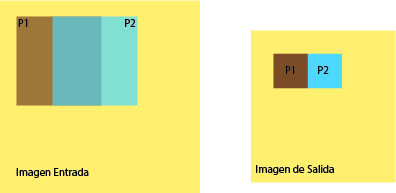
\includegraphics[scale=1]{img/prosImg.jpg}
			\caption{Proceso general de los kenels }
\end{figure}

\begin{figure}[h]
			\centering
				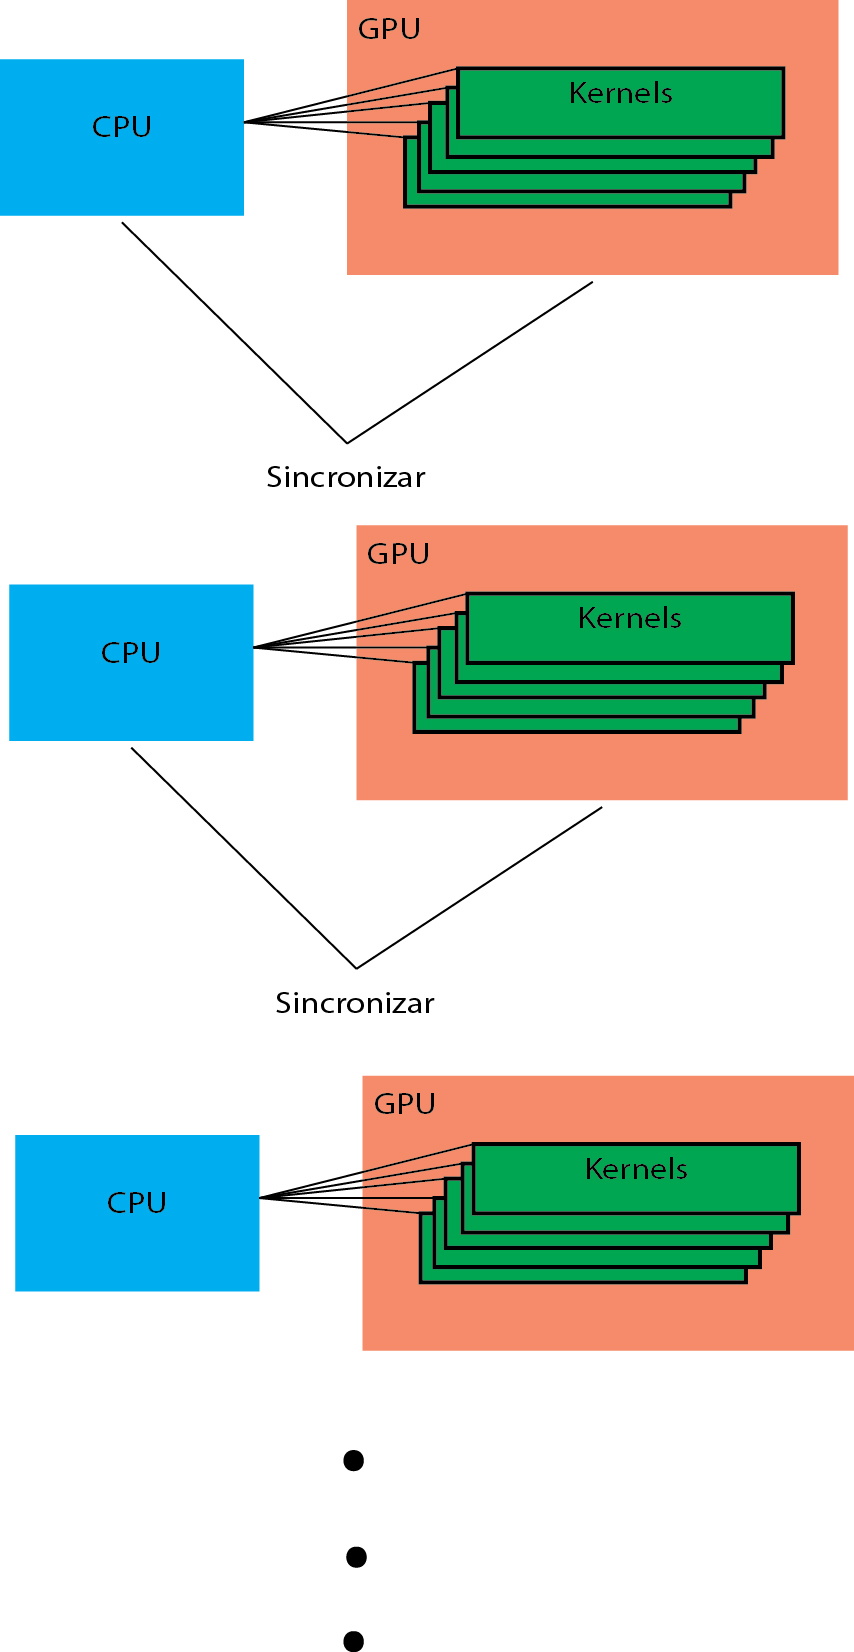
\includegraphics[scale=1]{img/lanzamiento.jpg}
			\caption{Lanzamiento de Kernels }
\end{figure}
\pagebreak

Cada uno de los kernels serán ejecutados múltiples veces, este trabajo sera desempeñado por el anfitrión (CPU) de forma secuencial, esto es importante ya que cada uno de estos kernels es lanzado sin importar que el anterior acabara de ejecutarse, si múltiples kernels son lanzados y tiene la misma especificación pero trabajan con diferentes secciones de los datos no existe problema. Pero si el anfitrión llegara a lanzar un kernel que tiene una especificación diferente a la de un banco de kernels iguales lanzados anteriormente y estos no han finalizado puede existir riesgo de corromper los datos. Entonces debemos de sincronizar , como se puede ver en la figura 4-5, al  dispositivo (GPU) con el anfitrión (CPU) para evitar caer en este tipo de errores.



\pagebreak
\section{Implementación}

Ahora que conocemos la estructura general de la solución, plantearé como construí cada una de las partes en las que dividí el algoritmo de SIFT, figura 4-3,  para poder adaptarlo a el modelo de programación de CUDA.

\subsection{Construcción del espacio escala y aproximación a un Laplaciano de Gaussiano}

Recordando un poco, el espacio escala se forma a partir de suavizar la imagen original a diferentes niveles de detalles, lo que hice fue cambiar el filtro gaussiano por uno que se aproximara a el Laplaciano de Gaussiana, que seria una diferencia de Gausianas. 

$$D(x,y;\sigma) = (G(x,y;k\sigma) - G(x,y;\sigma)) * I(x,y)$$ 

Para ello obtendremos los filtros Gaussianos con la ayuda de la librería OpenCV, y los restamos para así obtener los filtros que aplicaremos en cada octava. Quedando como los de las figura X-X.

///////////////////Imagen de DOG////////////////////////

También usaré OpenCV para cambiar el tamaño de las imágenes, para cada octava.

La sección de esta parte, de las que dividí el algoritmo, que es altamente paralelizable es al momento de hacer la convolución. Por este motivo lo que hice fue desarrollar un kernel, se puede encontrar en el apéndice A, que realice la convolución de una imagen y un filtro.

La idea es que estos kernels son lanzados por el anfitrión, se lanzaran tantos kernels como imágenes se necesitan para crear el espacio escala. Los kernels sera ejecutados de forma concurrente. 

La funcionalidad del kernel es, para cada pixel en la imagen de salida se asigna un hilo de diferentes bloques, y estos se encargaran con los datos de entrada, la imagen y el filtro, implementar la operación de convolución.\\

\begin{algorithm}[H]
\caption{Calculo de la convolución para cada imagen del espacio escala}
 \KwData{ImgEntrada, Filtro}
 \KwResult{Img }
 Para cada pixel en ImgEntrada asigna un hilo\;
 
 \ForAll{hilos}
 {
	\eIf{Img.pixel es orilla}
	{
		Img.pixel=0;
	}{
		
		Img.pixel= ImgEntrada.zona * Filtro; 
		\\
		\tcp{Donde * es el operador para la convolución}			
		}
 }
	

\end{algorithm}



EL resultado es como el de la figura X-X, tendremos imágenes muy similares para cada una de las octavas.

////////////////////Imagenes de una escala de la piramide////////////////////////
 
\subsection{Detección de puntos característicos}
En el espacio escala, obtenido anteriormente, buscaré los puntos extremos. A lo que nos referimos con esto es que en $D(x,y,\sigma)$ buscaré las ubicaciones máximas y mínimas, cada punto es comparado con sus ocho vecinos en la misma imagen y con sus otros dieciocho vecinos de escala, nueve en la imagen de arriba y nueve en la imagen de abajo. Solo se selecciona la ubicación si el pixel tiene un valor mayor o menor a todos sus vecinos.\\


\begin{algorithm}[H]
\caption{Búsqueda de puntos extremos}
 \KwData{ImgArriba, Img , ImgAbajo }
 \KwResult{ImgMascara}
 Para cada pixel en Img asigna un hilo\;
 
 \ForAll{hilos}
 {
	\eIf{Img.pixel es orilla}
	{
		ImgMascara.pixel=0\;
	}{
		\ForAll{pixel vecino a Img en ImgArriba, ImgAbajo e Img }
		{
			Compara cada pixel vecino con el pixel asignado al hilo\;
			\eIf{si todos los vecinos son menores o mayores}
			{
				ImgMascara.pixel = 1\;			
			}{
				ImgMascara.pixel = 0\;
			
			}
		
		}
		
	}
 }
	
\end{algorithm}


Como podemos ver en el algoritmo 2, lo que hacemos en el kernel es a cada hilo se le va a asignar un pixel de la imagen de entrada \texttt{Img} para compararla con sus vecinos y asi poder determinar si es un punto extremo. La imagen de salida terminara siendo una mascara binaria si existe un punto extremo, pondrá un pixel en blanco y donde no lo dejara en negro, como se muestra en la figura X-X; Podemos encontrar la implementación de este algoritmo en el apéndice B.


///////////////////////Mascara De imagen/////////////////////////////





\subsection{Eliminación de puntos característicos malos}

Ahora filtraré los puntos extremos que encontramos anteriormente. Existen dos casos donde los puntos extremos anteriormente seleccionados tendrían que ser eliminados:
	\begin{enumerate}
		\item El punto tiene un contraste muy bajo.
		\item El punto está localizado sobre un borde.
	\end{enumerate}		

\begin{algorithm}[H]
\caption{Eliminación de puntos característicos malos}
 \KwData{Img , ImgMascara}
 \KwResult{ImgMascara}
 Para cada pixel en Img asigna un hilo\;
 
 \ForAll{hilos}
 {
	\If{ImgMascara.pixel es mayor que 0}
	{
		\If{Img.pixel tiene contraste bajo o esta en un borde}
		{
			ImgMascara.pixel=0;
		}
	
				
	}
	
	
		
}
	
\end{algorithm}

Obtendremos una mascara muy parecida a la de la figura X-X pero esta vez tendremos muchos menos pixeles en color blanco. En el apéndice C podemos ver mas detalladamente como es que se realizo la implementación de esta parte de el algoritmo de SIFT.


///////////////////////Mascara De imagen  Filtrados   /////////////////////////////


\subsection{Asignación de orientación a los puntos característicos}

Encontrar la orientación de cada punto característico, basado en propiedades locales de la imagen, es importante para que el descriptor sea invariante a la rotación.


\begin{algorithm}[H]
\caption{Eliminación de puntos característicos malos}
 \KwData{Img}
 \KwResult{ImgMagnitud, ImgOrientacion}
 Para cada pixel en Img asigna un hilo\;
 
 \ForAll{hilos}
 {
	Calcular magnitud en Img.pixel\;
	Calcular orientación en Img.pixel\;
	
	ImgMagnitud.pixel= magnitud\;
	ImgOrientacion.pixel=orientación\;
	
}
\end{algorithm}



Para esta parte lo mejor fue dividir en dos kernels este proceso uno para calcular las magnitudes y orientaciones de los gradientes. En el apéndice D se encuentra la implementación de este kernel.

$$m(x,y) = \sqrt{ (L(x+1,y)-L(x-1,y))^2 + (L(x,y+1)-L(x,y-1))^2 }$$		
$$\theta(x,y) =  \tan^{-1} \left(\frac{L(x,y+1)-L(x,y-1)}{L(x+1,y)-L(x-1,y)}\right)$$

Y la otra sera donde tendremos que obtener los histogramas para cada punto característico y asignar una orientación dominante. En el apéndice E, encontraremos su implementación. 


\begin{algorithm}[H]
\caption{Eliminación de puntos característicos malos}
 \KwData{Img , ImgMascara, ImgMagnitud, ImgOrientacion}
 \KwResult{PuntosCaracteristicos}
 Para cada pixel en Img asigna un hilo\;
 
 \ForAll{hilos}
 {
	\If{ImgMascara.pixel es mayor que 0}
	{
		Realizar el histograma de a zona al rededor de el punto característico\;
		Encontrar cuales son los valores mas altos más altos\;
		Encontrar una orientación dominante con los puntos mas altos\;
		Almacenar la orientación y la ubicación de ese punto característico\; 
				
	}
	
	
		
}
	
\end{algorithm}
































%%\subsection{Generar Descriptor SIFT}
\pagebreak
\chapter{Pruebas y Resultados}
\spacing{1.5}
\section{Pruebas}
Para las pruebas realizadas se utilizó una computadora con un procesador AMD Phenom II 720 con tres núcleos a 2.80Ghz cada núcleo, 10 GB de memoria RAM y una tarjeta gráfica NVIDIA GeForce GTX 650 Ti tiene una arquitectura Kepler con 768 núcleos CUDA, memoria de 2 GB y un ancho de banda para 86.4 GB/s. En cuanto al software las pruebas de hicieron bajo un sistema operativo xubuntu 14.04, utilizando openCV y CUDA 6.5.\\
Teniendo en cuenta el hardware y la forma en que se diseñaron los kernels se deben realizar ciertas optimizaciones. Para esta implementación como no se usa memoria compartida le daremos preferencia a la memoria cache L1 usando, la función \textbf{cudaFuncSetCacheConfig()} recibe 2 parámetros el primero será el nombre de la función del dispositivo (kernel) y el segundo es la configuración que se le dará a la memoria, en este caso \textit{cudaFuncCachePreferL1}. Además, se debe tomar en cuenta la ocupación de los SM definida por la relación entre los \textit{warps} activos y la cantidad de \textit{warps} por SM. NVIDIA desarrollo una herramienta llamada CUDA Occupancy Calculator\cite{calc}, la cual auxilia al desarrollador a encontrar la máxima ocupación para el lanzamiento de un kernel. Necesitará como datos de entrada el número de hilos por bloque, la cantidad de memoria compartida usada y el número de registros por hilo.\\\\\\
Otra herramienta que resulta muy útil para identificar problemas de rendimiento es el perfilador visual de NVIDIA\cite{profile}, gracias a este se pudo analizar la ocupación teórica calculada contra la real para cada ejecución de los diferentes kernel lanzados con diferentes imágenes de entrada, como se puede ver en la tabla 5-1.\\
\begin{table}[H]
\centering
\begin{tabular}{|l|c|c|c|}
\hline
\multicolumn{4}{|c|}{Ocupación de los SM} \\
\cline{1-4}
Kernel & Teórica &  Máxima Real &  Mínima Real\\
\hline \hline
 Convolución                    & 100\%   &  99\%   &   13\%                     \\ \cline{1-4}
 Localización de min-max        & 100\%   &  93\%   &   12\% \\ \cline{1-4}
 Remover puntos malos           & 100\%   &  93\%   &   28\%                \\ \cline{1-4}
 Asignar magnitud y orientación & 100\%   &  84\%   &   32\%            \\ \cline{1-4}
 Puntos característicos         & 56\%    &  55\%   &   1.7\%           \\ \cline{1-4}
\end{tabular}
\caption{Ocupación teórica vs ocupación real}
\label{tabla:final}
\end{table}
Una vez dicho como se encontró la mejor condición de lanzamiento y distribución de la memoria para cada kernel, se puede describir como se realizaron las pruebas en general. Las pruebas se realizaron tomando un grupo de imágenes de diferentes resoluciones como entrada de la implementación propuesta, para medir el tiempo que le tomaba procesar la imagen y compararlo con otras implementaciones del algoritmo SIFT, ya existentes. La razón de porque imágenes de distintas resoluciones es por la manera tan diversa de obtener imágenes en el robot Justina.\\\\\\\\\\\\
\section{Resultados}
Hay dos imágenes que fueron las que ayudaron a realizar paso a paso el desarrollo de la implementación propuesta, la primera imagen es un castor, y la segunda imagen de un gato (figura 5-1). La razón por la cual se tomaron estas dos imágenes fue porque la imagen del castor es una imagen pequeña con pocos puntos característicos, y la del gato siendo de una resolución mayor y con una gran cantidad de puntos característicos. Siendo estas dos imágenes los extremos en cuanto a los datos de entrada.\\

\begin{figure}[H]
    \centering
    \begin{subfigure}[b]{0.4\textwidth}
        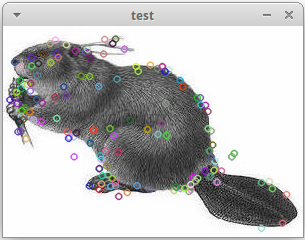
\includegraphics[width=\textwidth]{img/castor.png}
        \caption{Castor}
    \end{subfigure}
    ~ %add desired spacing between images, e. g. ~, \quad, \qquad, \hfill etc. 
      \begin{subfigure}[b]{0.4\textwidth}
        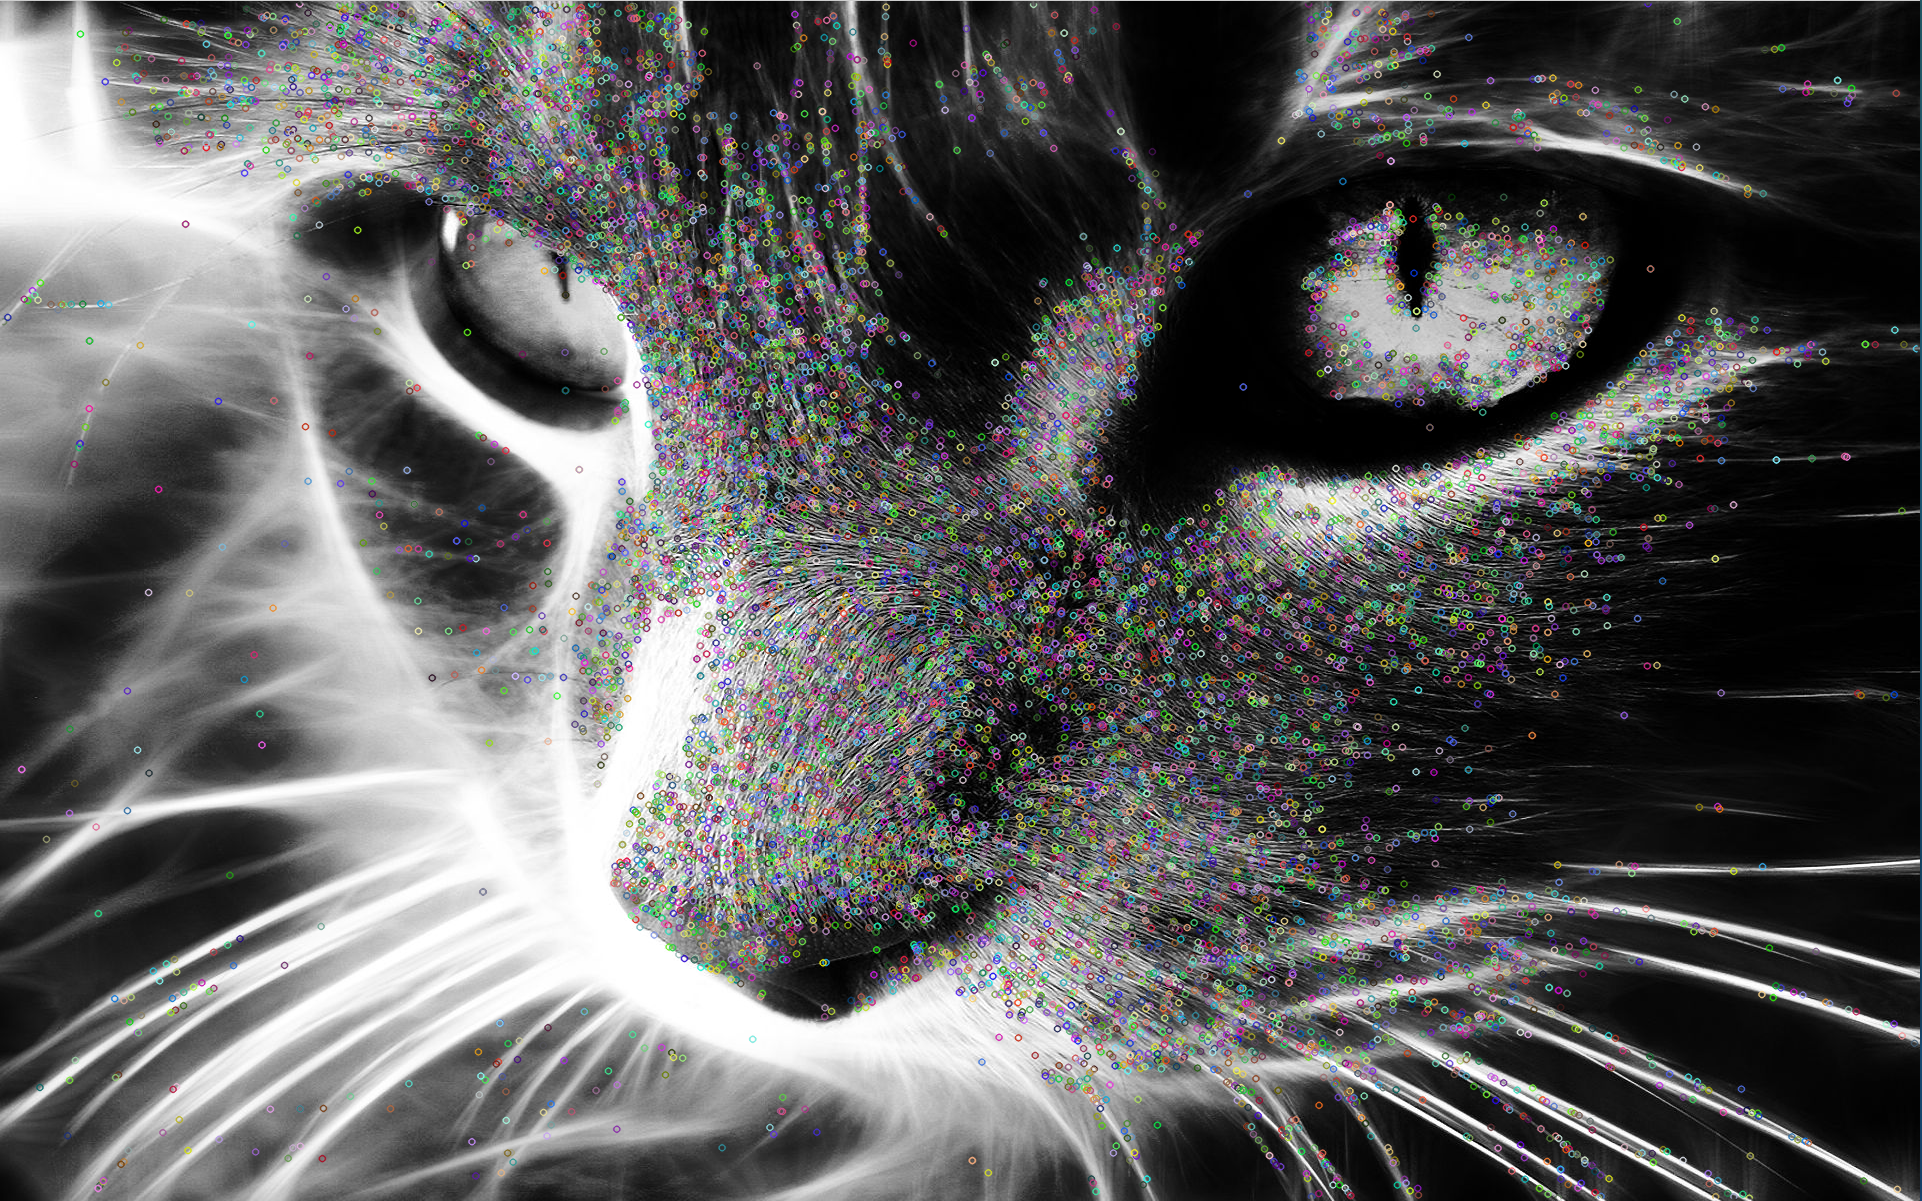
\includegraphics[width=\textwidth]{img/gato.png}
        \caption{Gato}
    \end{subfigure}
    \caption{Puntos característicos encontrados }
\end{figure}



La primer prueba que se hizo con el castor y el gato, consistió en medir el tiempo que tardaban en ejecutarse ciertas secciones del código de una implementación abierta de SIFT llamada Open SIFT \cite{OpenSIFT}, la cual se usa para la detección de objetos en el robot Justina, y en la implementación de SIFT con CUDA realizada para obtener los puntos característicos. Se puede observar en las tablas 5-2 y 5-3 los resultados de estas pruebas.\\
\begin{table}[H]
\centering
\begin{tabular}{|l|c|c|}
\hline
\multicolumn{3}{|c|}{Castor} \\
\cline{1-3}
Partes de SIFT & CUDA SIFT & Open SIFT\\
\hline \hline
 Espacio escala DoG      & 17.25 ms   &  29.32 ms                        \\ \cline{1-3}
 Detección y filtrado de PC & 2.62 ms   &  50.09 ms    \\ \cline{1-3}
 Orientación de PC       & 8.80 ms   &  12.35 ms                        \\ \cline{1-3}
\end{tabular}
\caption{La resolución de la imagen es de 300x211 px y se encontraron 120 puntos característicos}
\label{tabla:final}
\end{table}
\begin{table}[H]
\centering
\begin{tabular}{|l|c|c|}
\hline
\multicolumn{3}{|c|}{Gato} \\
\cline{1-3}
Partes de SIFT & CUDA SIFT & Open SIFT\\
\hline \hline
 Espacio escala DoG         & 473.33 ms  &  957.19 ms                       \\ \cline{1-3}
 Detección y filtrado de PC & 65.29 ms   &  2210.82 ms                       \\ \cline{1-3}
 Orientación de PC          & 125.2 ms   &  1014.89 ms                      \\ \cline{1-3}
\end{tabular}
\caption{La resolución de la imagen es de 1920x1200 px y se encontraron 12000 puntos característicos}
\label{tabla:final}
\end{table}
Lo que se hizo después, fue medir el tiempo para obtener los puntos característicos en 3 diferentes implementaciones, la desarrollada para CUDA, la de OpenSIFT y por último la que se encuentra en OpenCV. Se pueden ver los resultados y el desempeño que se obtuvo en la tabla 5-4.\\
\begin{table}[H]
\centering
\begin{tabular}{|c|c|c|c|c|}
\hline
\multicolumn{5}{|c|}{Castor} \\
\cline{1-5}
Resolución & CUDA SIFT & Open SIFT & Opencv SIFT & Puntos Característicos \\
\hline \hline
320 x 240 px & 31.87 ms   &   93.22 ms  &  49.42 ms   & 120\\ \cline{1-5}
\hline \hline
\multicolumn{5}{|c|}{Gato} \\
\cline{1-5}
Resolución & CUDA SIFT & Open SIFT & Opencv SIFT & Puntos Característicos \\
\hline \hline
1920x1200 px & 676.32 ms &  4221.41 ms & 1415.98 ms   & 12000\\ \cline{1-5}
\end{tabular}
\caption{Tiempo de ejecución de la implementación en paralelo y 2 más de forma secuencial}
\label{tabla:final}
\end{table}
\begin{table}[H]
\centering
\begin{tabular}{|c|c|c|c|c|}
\hline
\multicolumn{3}{|c|}{Castor} \\
\cline{1-3}
Resolución &  Open SIFT/CUDA SIFT & Opencv SIFT/CUDA SIFT  \\
\hline \hline
320 x 240 px & 2.92 & 1.55 \\ \cline{1-3}
\hline \hline
\multicolumn{3}{|c|}{Gato} \\
\cline{1-3}
Resolución & Open SIFT/CUDA SIFT & Opencv SIFT/CUDA SIFT\\
\hline \hline
1920x1200 px  & 6.24 & 2.09 \\ \cline{1-3}
\end{tabular}
\caption{ Speedup entre la implementación en paralelo y 2 más de forma secuencial}
\label{tabla:final}
\end{table}
Estas imágenes no eran las más adecuadas para hacer pruebas, ya que el robot de servicio Justina trabaja con imágenes como las de la figuras 5-3. Las primeras tres son objetos que tiene que manipular.\\
\begin{figure}[H]
    \centering
    \begin{subfigure}[b]{0.3\textwidth}
        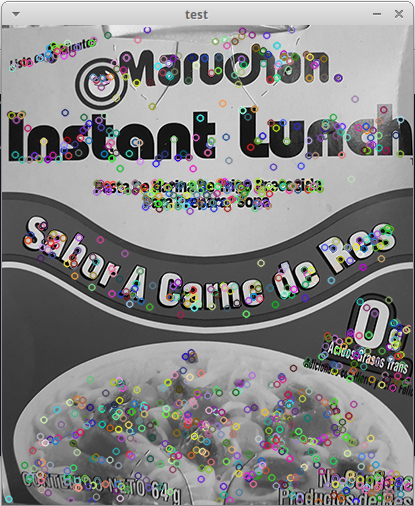
\includegraphics[width=\textwidth]{img/sopa.png}
        \caption{Sopa}
    \end{subfigure}
    ~ %add desired spacing between images, e. g. ~, \quad, \qquad, \hfill etc. 
      \begin{subfigure}[b]{0.2\textwidth}
        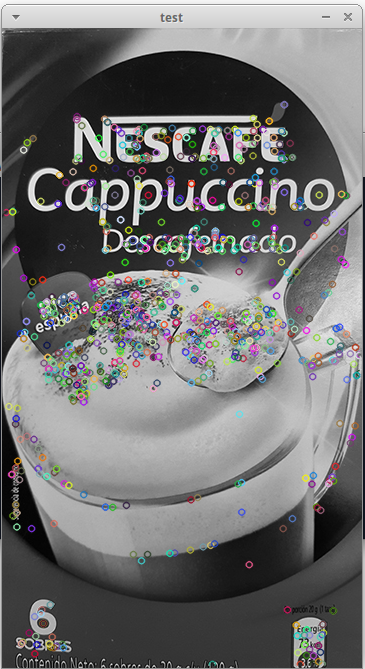
\includegraphics[width=\textwidth]{img/cafe.png}
        \caption{Café}
    \end{subfigure}

    \begin{subfigure}[b]{0.35\textwidth}
        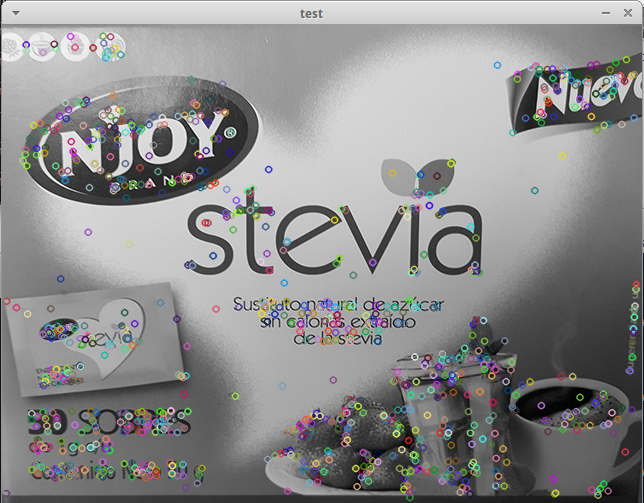
\includegraphics[width=\textwidth]{img/stevia.png}
        \caption{Stevia}
    \end{subfigure}
    ~ %add desired spacing between images, e. g. ~, \quad, \qquad, \hfill etc. 
      \begin{subfigure}[b]{0.35\textwidth}
        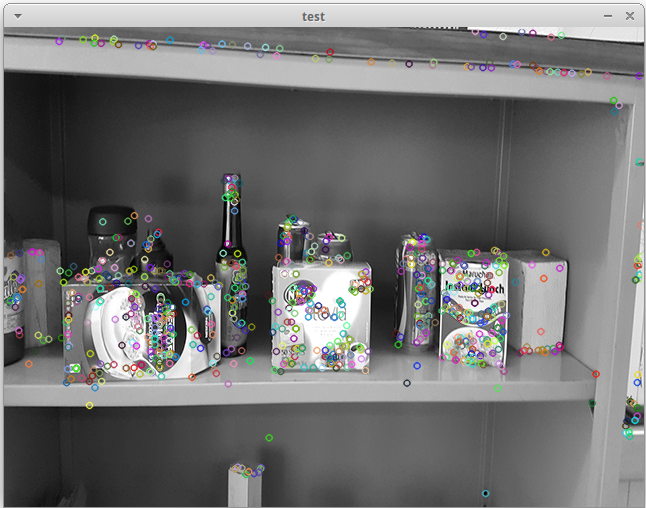
\includegraphics[width=\textwidth]{img/estante.png}
        \caption{Estante}
    \end{subfigure}
    \caption{Puntos característicos encontrados}
\end{figure}
Lo que se hizo fue medir cuánto tiempo se tardaban en generar los puntos característicos en las 3 implementaciones anteriormente mencionadas y cambiar las resoluciones de estas imágenes, porque el robot no siempre vera los objetos del mismo tamaño. Dependerá de la cámara que se esté usando o que tan lejos esté viendo los objetos. Los resultados los podemos ver a continuación en las siguientes tablas:
\begin{table}[phtb]
\centering
\begin{tabular}{|c|c|c|c|c|}
\hline
\multicolumn{5}{|c|}{Stevia} \\
\cline{1-5}
Resolución & CUDA SIFT & Open SIFT & Opencv SIFT & Puntos Característicos\\
\hline \hline
 320 x 240 px  & 31.87 ms   &   151.10 ms  &  49.42 ms   & 370\\ \cline{1-5}
 640 x 480 px  & 97.91 ms   &   484.64 ms  &  182.46 ms  & 920\\ \cline{1-5}
1280 x 960 px  & 335.05 ms  &  1751.10 ms  &  679.60 ms  & 2800\\ \cline{1-5}
2560 x 1920 px & 1251.38 ms &  5911.26 ms  &  2893.68 ms & 3000\\ \cline{1-5}
\end{tabular}
\caption{Tiempo de ejecución de la implementación en paralelo y 2 más de forma secuencial}
\label{tabla:final}
\end{table}
\begin{table}[phtb]
\centering
\begin{tabular}{|c|c|c|c|c|}
\hline
\multicolumn{3}{|c|}{Stevia} \\
\cline{1-3}
Resolución & Open SIFT/CUDA SIFT & Opencv SIFT/CUDA SIFT \\
\hline \hline
 320 x 240 px  &  4.74  &  1.55   \\ \cline{1-3}
 640 x 480 px  &  4.94  &  1.86  \\ \cline{1-3}
1280 x 960 px  &  5.22  &  2.02  \\ \cline{1-3}
2560 x 1920 px &  4.72  &  2.31 \\ \cline{1-3}
\end{tabular}
\caption{Speedup la implementación en paralelo y 2 más de forma secuencial}
\label{tabla:final}
\end{table}

\begin{table}[phtb]
\centering
\begin{tabular}{|c|c|c|c|c|}
\hline
\multicolumn{5}{|c|}{Café} \\
\cline{1-5}
Resolución & CUDA SIFT & Open SIFT & Opencv SIFT & Puntos Característicos\\
\hline \hline
 320 x 180 px  & 30.25 ms  &  117.95 ms  & 39.25 ms   & 290\\ \cline{1-5}
 640 x 360 px  & 81.91 ms  &  484.64 ms  & 182.46 ms  & 760\\ \cline{1-5}
1280 x 720 px  & 284.57 ms &  1415.27 ms & 518.27 ms  & 2800\\ \cline{1-5}
2560 x 1440 px & 993.96 ms &  4963.27 ms & 1951.21 ms & 7000\\ \cline{1-5}
\end{tabular}
\caption{Tiempo de ejecución de la implementación en paralelo y 2 más de forma secuencial}
\label{tabla:final}
\end{table}

\begin{table}[phtb]
\centering
\begin{tabular}{|c|c|c|c|c|}
\hline
\multicolumn{3}{|c|}{Café} \\
\cline{1-3}
Resolución & Open SIFT/CUDA SIFT & Opencv SIFT/CUDA SIFT \\
\hline \hline
 320 x 240 px  & 3.89   &  1.29   \\ \cline{1-3}
 640 x 480 px  & 5.91   &  2.22  \\ \cline{1-3}
1280 x 960 px  & 4.97   &  1.82  \\ \cline{1-3}
2560 x 1920 px & 4.99   &  1.96 \\ \cline{1-3}
\end{tabular}
\caption{Speedup la implementación en paralelo y 2 más de forma secuencial}
\label{tabla:final}
\end{table}

\begin{table}[phtb]
\centering
\begin{tabular}{|c|c|c|c|c|}
\hline
\multicolumn{5}{|c|}{Sopa} \\
\cline{1-5}
Resolución & CUDA SIFT & Open SIFT & Opencv SIFT & Puntos Característicos\\
\hline \hline
 206 x 240 px  & 28.10 ms  &  130.98 ms  & 37.78 ms   & 425\\ \cline{1-5}
 411 x 480 px  & 74.43 ms  &  412.04 ms  & 129.49 ms  & 1000\\ \cline{1-5}
 802 x 906 px  & 241.83 ms &  1400.59 ms & 469.07 ms  & 3000\\ \cline{1-5}
1645 x 1920 px & 850.29 ms &  4478.54 ms & 1674.67 ms & 3900\\ \cline{1-5}
\end{tabular}
\caption{Tiempo de ejecución de la implementación en paralelo y 2 más de forma secuencial}
\label{tabla:final}
\end{table}

\begin{table}[phtb]
\centering
\begin{tabular}{|c|c|c|c|c|}
\hline
\multicolumn{3}{|c|}{Sopa} \\
\cline{1-3}
Resolución & Open SIFT/CUDA SIFT & Opencv SIFT/CUDA SIFT \\
\hline \hline
 320 x 240 px  &  4.66  &  1.34   \\ \cline{1-3}
 640 x 480 px  &  5.54  &  1.73  \\ \cline{1-3}
1280 x 960 px  &  5.79  &  1.93  \\ \cline{1-3}
2560 x 1920 px &  5.26  &  1.96 \\ \cline{1-3}
\end{tabular}
\caption{Speedup la implementación en paralelo y 2 más de forma secuencial}
\label{tabla:final}
\end{table}

\begin{table}[phtb]
\centering
\begin{tabular}{|c|c|c|c|c|}
\hline
\multicolumn{5}{|c|}{Estante} \\
\cline{1-5}
Resolución & CUDA SIFT & Open SIFT & Opencv SIFT & Puntos Característicos\\
\hline \hline
 320 x 240 px  & 33.45 ms   & 130.24 ms   & 47.52 ms   & 210\\ \cline{1-5}
 640 x 480 px  & 101.20 ms  &  451.39 ms  & 177.28 ms  & 700\\ \cline{1-5}
1280 x 960 px  & 340.92 ms  &  1602.51 ms & 669.09 ms  & 2100\\ \cline{1-5}
2560 x 1920 px & 1275.37 ms &  6031.39 ms & 3037.60 ms & 3700\\ \cline{1-5}
\end{tabular}
\caption{Tiempo de ejecución de la implementación en paralelo y 2 más de forma secuencial}
\label{tabla:final}
\end{table}
\begin{table}[phtb]
\centering
\begin{tabular}{|c|c|c|c|c|}
\hline
\multicolumn{3}{|c|}{Estante} \\
\cline{1-3}
Resolución & Open SIFT/CUDA SIFT & Opencv SIFT/CUDA SIFT \\
\hline \hline
 320 x 240 px  &  3.89  &  1.42   \\ \cline{1-3}
 640 x 480 px  &  4.46  &  1.75  \\ \cline{1-3}
1280 x 960 px  &  4.70  &  1.96  \\ \cline{1-3}
2560 x 1920 px &  4.73  &  2.38 \\ \cline{1-3}
\end{tabular}
\caption{Speedup la implementación en paralelo y 2 más de forma secuencial}
\label{tabla:final}
\end{table}
\pagebreak
Un factor que pudo afectar el tiempo de ejecución de todos los programas fue la cantidad de puntos característicos que existen en la imagen, cosa que no pasó. Se puede observar cómo se repite el fenómeno que notamos con el castor y el gato. Entre más grande es la imagen obtenemos un desempeño más grande, esto paso para todos los casos en las imágenes anteriores. Es importante mencionar que el tiempo medido en las tablas incluye el cuello de botella que existe al estar pasando datos de la memoria RAM de la computadora a la memoria de la GPU.

\pagebreak
 
 
 \chapter{Conclusiones y Trabajo a Futuro}

\section{Conclusiones}

 Las pruebas a las que es sometido el robot de servicio Justina son más rigurosas, por este motivo los sistemas deben ser cada vez más rápidos y confiables. También las nuevas generaciones de sensores son mucho mejores tenemos más información para analizar, actualmente se utiliza un sensor Kinect para obtener las imágenes, esta tiene una resolución de  640 x 480 px y se utiliza el código de openSIFT para procesar esta imágenes, después     se adquirió una cámara RGB Logitech C920 que tiene una  de 1920 x 1080 px, el procesamiento de la imagen fue mucho más lento. Se planea empezar a usar también el nuevo sensor de Microsoft Kinect 2 el cual también tiene una resolución de 1920 x 1080 px. 
 
 
 Los resultados obtenidos tiene dos matices en mi opinion, donde las imágenes son muy pequeñas y hay poco que procesar , cuando el robot necesita encontrar objetos en una mesa, segmenta los objetos de la mesa y quedan solo los objetos, que no tienen una cantidad muy grande de pixeles a procesar, por lo que aun que es un poco más rápido procesarlos en el GPU, no tiene gran aceleración en comparación a la librería de OpenCV y es mucho más sencillo implementarlo; la otra parte es que se ha estado trabajando para que Justina no solo encuentre objetos en la mesa sino que debe tener capacidad para encontrarlos en un libreo o estante. En el laboratorio de BioRobotica de la UNAM  se ha estado tratando de segmentar estos estantes o libreros para poder seguir con la misma metodología al momento de buscar objetos, cosa que no se ha logrado con éxito total. Lo que se implemento fue hacer una búsqueda de los objetos en toda la imagen, para esto se intentó hacer con las imágenes que entrega el Kinect, pero la baja calidad de la imagen no permitía encontrar los objetos, ya que la distancia de donde se tomaba la foto era más lejos de lo que acostumbra ser.
 Se cambió la fuente de la imagen por la cámara C920 y los resultados mejoraron, pero el tiempo de procesamiento aumento.

 EL robot Justina participa en una competencia principalmente llamada Robocup, en 2015 se puso una nueva prueba llamada  \textit{Manipulation and object recognition} donde se tenía que buscar objetos en un librero y manipularlos básicamente. Para esta prueba solo dan 3 minutos para reconocer y manipular objetos,  de los cuales nosotros gastamos todo el tiempo solo reconociendo, ya que con una sola foto no podríamos analizar todos los objetos que  hay en el librero, por lo cual hay que hacer varias tomas de diferente ángulos.


 
 El punto a resaltar es que la cantidad de datos que se tienen que procesar crecieron solo tres veces y se tarda en procesar hasta 13 veces más tiempo que con las anteriores resoluciones, lo que empieza a sonar como una buena idea es voltear a ver a las tarjetas gráficas de propósito general, las cuales ya se cuentan con ellas en las laptops que el robot usa. Observando los resultados con resoluciones de 1920 x 1080 podemos ver una aceleración de hasta 5 veces respecto a OpenSIFT y 2 veces contra la librería OpenCV, ya que en lugar de que el proceso tarde 5 segundos por foto estaría tardando solo un segundo.  
 

\section{Trabajo a Futuro}

 Como se vio hay nuevas necesidades para este Robot Justina, y con un aceleramiento de 5 veces no me parece suficiente  por lo que hay que seguir trabajando en esto. Hay que hacer pruebas en diferentes tarjetas gráficas más poderosas y de nueva generación.

 Pero no solo el hardware es lo que hay que probar, como vimos en el capítulo tres, los diferentes tipos de memoria ayudan a hacer más eficiente el acceso a los datos, experimentar con estos tipos de memoria para buscar un mejor desempeño. Otro aspecto que se podría mejorar es al momento de lanzar el Kernel ya que hay que buscar cual es la configuración adecuada para el lanzamiento, con esto me refiero al número de bloques e hilos que ejecutaran el programa. 

 Encontrar otra forma más rápida de pasar los datos de la memoria RAM a la memoria de la GPU ya que ese es un cuello de botella importante, encontrar otra forma de manejar las imágenes para que los accesos a memoria será más rápidos. En fin tratar de sacarle todo el jugo a la tarjeta gráfica adaptando el código a esta.  

 Algo que ayudaría a Justina, es desarrollar el algoritmo para que genere el descriptor de SIFT y otro para hacer el emparejamiento de estos descriptores en paralelo, no sé si usar las tarjetas gráficas para hacer el emparejamiento sea lo óptimo pero igual se puede intentar y ver si arroja resultados favorables.  
 
 



\appendix

\chapter{Kernel Convolución}
\begin{small}



\lstset{language=C,
                basicstyle=\ttfamily,
                keywordstyle=\color{blue}\ttfamily,
                stringstyle=\color{red}\ttfamily,
                commentstyle=\color{green}\ttfamily,
        frame= single,
        numbers = none,
        xleftmargin=0.5em,
        framexleftmargin=0.5em        
}
\begin{lstlisting}
__global__ void Convolution(float* image,float* mask, 
		ArrayImage* PyDoG, int maskR,int maskC,
	        int imgR,int imgC, float* imgOut, int idxPyDoG)
{
int tid= threadIdx.x;
int bid= blockIdx.x;
int bDim=blockDim.x;
int gDim=gridDim.x;
int iImg=0;
float aux=0;
int pxlThrd = ceil((double)(imgC*imgR)/(gDim*bDim)); 
for(int i = 0; i <pxlThrd; ++i)
	{
		
iImg=(tid+(bDim*bid)) + (i*gDim*bDim); 
 if(iImg < imgC*imgR){
  int condition=maskC/2+imgC*(floor((double)maskC/2));
  if (iImg-condition < 0  ||										
	 iImg+condition > imgC*imgR ||								
	 iImg%imgC < maskC/2 ||										
	 iImg%imgC > (imgC-1)-(maskC/2) )							
	 {
	 	aux=0;
	 }else{		
		int itMask = 0;
		int itImg=iImg-condition;
		for (int j = 0; j < maskR; ++j)
		{		
			for (int h = 0; h < maskC; ++h)
			{
				aux+=image[itImg]*mask[itMask];
				++itMask;
				++itImg;
			}
			itImg+=imgC-maskC;
		}
	 }
	imgOut[iImg]=aux;
	aux=0;
  }
 }
 PyDoG[idxPyDoG].image=imgOut;
}
\end{lstlisting}

\end{small}
\pagebreak

\chapter{Kernel Localización de máximos y mínimos }

\begin{small}
\lstset{language=C,
                basicstyle=\ttfamily,
                keywordstyle=\color{blue}\ttfamily,
                stringstyle=\color{red}\ttfamily,
                commentstyle=\color{green}\ttfamily,
        frame= single,
        numbers = none,
        xleftmargin=0.5em,
        framexleftmargin=0.5em        
}
\begin{lstlisting}
__global__ void LocateMaxMin(ArrayImage* PyDoG, int idxPyDoG ,
		float * imgOut ,MinMax * mM, int maskC, int imgR,
		int imgC, int idxmM)
{
int tid= threadIdx.x;
int bid= blockIdx.x;
int bDim=blockDim.x;
int gDim=gridDim.x;
int iImg=0;
int pxlThrd = ceil((double)(imgC*imgR)/(gDim*bDim)); 
for(int i = 0; i <pxlThrd; ++i)
 {
  int min=0;
  int max=0;
  float value=0.0;
  float compare =0.0;
  iImg=(tid+(bDim*bid)) + (i*gDim*bDim); 
  if(iImg < imgC*imgR){
	int condition=maskC/2+imgC*(floor((double)maskC/2));
	if (iImg-condition < 0  ||										
		iImg+condition > imgC*imgR ||								
		iImg%imgC < maskC/2 ||										
		iImg%imgC > (imgC-1)-(maskC/2) )							
	{                  
		imgOut[iImg]=0;				
	}
	else{
		value=PyDoG[idxPyDoG].image[iImg];
		for (int m = -1; m < 2; ++m)
		{
		  int itImg=iImg-(1+imgC);
		  for (int j = 0; j < 3; ++j)
		  {		
		    for (int h = 0; h < 3; ++h)
			{
				compare =PyDoG[idxPyDoG+m].image[itImg];
				if(value<=compare && max==0)
				{
					++min;
				}
				else if(value>=compare && min==0)
				{
					++max;
				}
				++itImg;
			  }
			  itImg+=imgC-3;
		  }
		}
 		if( (min==26 || max==26)) {
			imgOut[iImg]=1;
		}else{
			imgOut[iImg]=0;
		}
	}
  }
 }
mM[idxmM].minMax=imgOut;
}
\end{lstlisting}

\end{small}
\pagebreak
\chapter{Kernel Remover puntos malos}

\begin{small}
\lstset{language=C,
                basicstyle=\ttfamily,
                keywordstyle=\color{blue}\ttfamily,
                stringstyle=\color{red}\ttfamily,
                commentstyle=\color{green}\ttfamily,
        frame= single,
        numbers = none,
        xleftmargin=0.5em,
        framexleftmargin=0.5em        
}
\begin{lstlisting}
__global__ void RemoveOutlier(ArrayImage* PyDoG, MinMax * mM,
	int idxmM, int idxPyDoG, int imgR,int imgC ,float* auxOut)
{
int tid= threadIdx.x;
int bid= blockIdx.x;
int bDim=blockDim.x;
int gDim=gridDim.x;
int iImg=0;
int pxlThrd = ceil((double)(imgC*imgR)/(gDim*bDim)); 
for(int i = 0; i <pxlThrd; ++i 
{

  iImg=(tid+(bDim*bid)) + (i*gDim*bDim); 
		
  if(iImg < imgC*imgR){
	if(mM[idxmM].minMax[iImg]>0 && PyDoG[idxPyDoG].image[iImg]>0.05)
	{
	  float d, dxx, dyy, dxy, tr, det;
	  d = PyDoG[idxPyDoG].image[iImg];
	  dxx = PyDoG[idxPyDoG].image[iImg+1]+
	  	PyDoG[idxPyDoG].image[iImg-1] - (2*d);
	  dyy = PyDoG[idxPyDoG].image[iImg+imgC]+
	  	PyDoG[idxPyDoG].image[iImg-imgC] - (2*d);
	  dxy = (PyDoG[idxPyDoG].image[iImg+1+imgC]-
	  	PyDoG[idxPyDoG].image[iImg-1+imgC] - 
	  	PyDoG[idxPyDoG].image[iImg+1-imgC] +
	  	PyDoG[idxPyDoG].image[iImg-1-imgC])/4.0;
	  tr = dxx + dyy;
	  det = dxx*dyy - dxy*dxy;
		
	  if(det<=0 && !(tr*tr/det < 12.1))
	  mM[idxmM].minMax[iImg]=0;
	 }else
	 {
	   mM[idxmM].minMax[iImg]=0;
	 }
     auxOut[iImg]=mM[idxmM].minMax[iImg];
	}
}
	
}
\end{lstlisting}

\end{small}
\pagebreak

\chapter{Kernel Asignar magnitud y orientación}

\begin{small}
\lstset{language=C,
                basicstyle=\ttfamily,
                keywordstyle=\color{blue}\ttfamily,
                stringstyle=\color{red}\ttfamily,
                commentstyle=\color{green}\ttfamily,
        frame= single,
        numbers = none,
        xleftmargin=0.5em,
        framexleftmargin=0.5em        
}
\begin{lstlisting}
__global__ void OriMag(ArrayImage* PyDoG, int idxPyDoG,
	int imgR,int imgC , ArrayImage* Mag, ArrayImage* Ori,
	int idxMagOri, float* MagAux, float* OriAux) 
{
int tid= threadIdx.x;
int bid= blockIdx.x;
int bDim=blockDim.x;
int gDim=gridDim.x;
float dx,dy;
int iImg=0;
int pxlThrd = ceil((double)(imgC*imgR)/(gDim*bDim)); 
for(int i = 0; i <pxlThrd; ++i)
{
	iImg=(tid+(bDim*bid)) + (i*gDim*bDim); 
	if(iImg < imgC*imgR){
	int condition=1/2+imgC*(floor((double)1/2));
	if (iImg-condition < 0  ||										
	iImg+condition > imgC*imgR ||								
	iImg%imgC < 1/2 ||										
	iImg%imgC > (imgC-1)-(1/2) )							
	{                  
		OriAux[iImg]=0;
		MagAux[iImg]=0;
	}
	else{
		dx=PyDoG[idxPyDoG].image[iImg+1]-
			PyDoG[idxPyDoG].image[iImg-1];
		dy=PyDoG[idxPyDoG].image[iImg+imgC]-
			PyDoG[idxPyDoG].image[iImg-imgC];
		MagAux[iImg]=sqrt(dx*dx + dy*dy);
		OriAux[iImg]=atan2(dy,dx);
    }
}
}
	
	Mag[idxMagOri].image= MagAux;
	Ori[idxMagOri].image= OriAux;

	
}
\end{lstlisting}


\end{small}
\pagebreak
\chapter{Kernel Generar puntos característicos}
\begin{small}

	\lstset{language=C,
                basicstyle=\ttfamily,
                keywordstyle=\color{blue}\ttfamily,
                stringstyle=\color{red}\ttfamily,
                commentstyle=\color{green}\ttfamily,
        frame= single,
        numbers = none,
        xleftmargin=0.5em,
        framexleftmargin=0.5em        
}
\begin{lstlisting}
__global__ void KeyPoints(ArrayImage * Mag,
	ArrayImage * Ori, MinMax * mM , int idxMOmM,
	keyPoint * KP, float sigma, int imgR,int imgC,
	int octava )
{
int tid= threadIdx.x;
int bid= blockIdx.x;
int bDim=blockDim.x;
int gDim=gridDim.x;
float o = 0;
int x=0, y=0, octv=-1;
int iImg=0;
int pxlThrd = ceil((double)(imgC*imgR)/(gDim*bDim)); 
for(int i = 0; i <pxlThrd; ++i) 
{
	iImg=(tid+(bDim*bid)) + (i*gDim*bDim);  
	octv=-1;
	if(iImg < imgC*imgR ){
	  if(mM[idxMOmM].minMax[iImg]>0){
		int condition=9/2+imgC*(floor((double)9/2));
		if (iImg-condition < 0  ||														iImg+condition > imgC*imgR ||												iImg%imgC < 9/2 ||										
			iImg%imgC > (imgC-1)-(9/2) )							
		{                  
		  o=-1.0;
		  x=-1;
		  y=-1;
		  octv=-1;
		}
		else{
		  float histo[36]={0,0,0,0,0,0,0,0,0,0,0,0,0,0,0,0,0,0,0,
		  	0,0,0,0,0,0,0,0,0,0,0,0,0,0,0,0,0};
		  octv=octava;
		  x=iImg%imgC;
		  y=iImg/imgC;
		  int idxMO= (iImg-4)-(4*imgC);
		  float exp_denom = 2.0 * sigma * sigma;
		  float w;
		  int bin;
		  for (int i = -4; i < 5; ++i)
		  {
		    for (int j = -4; j < 5; ++j)
			{
			  w = exp( -( i*i + j*j ) / exp_denom );
			  bin=round((double)(36*Ori[idxMOmM].image[idxMO])
			  			/6.28318530718);
	  		  bin = ( bin < 36 )? bin : 0;
	  		  histo[bin]= w*Mag[idxMOmM].image[idxMO];
	  		  ++idxMO;
			 }
			 idxMO=idxMO+imgC-9;
		   }
		   int idxH=0;
		   float valMaxH = histo[0];
		   for (int i = 1; i < 36; ++i)
		   {
		    if(histo[i]>valMaxH){
		      idxH = i;
		    }
		   }
		   int l = (idxH == 0)? 35:idxH-1;
		   int r = (idxH+1)%36;
		   float bin_= bin + ((0.5*(histo[l]-histo[r]))/
		   		(histo[l]-(2*histo[idxH])+histo[r]));
		   bin_= ( bin_ < 0 )? 36 + bin_ :
		   ( bin_ >= 36 )? bin_ - 36 :
		   bin_;
		   o=((6.28318530718*bin_)/36)-3.141592654;
	    }
	  }
	  KP[iImg].orientacion=o;
	  KP[iImg].x=x;
	  KP[iImg].y=y;
	  KP[iImg].octv=octv;
	}
}
}
\end{lstlisting}

\end{small}
\pagebreak
%%\chapter{Kernel Generar descriptor}






\cleardoublepage
\phantomsection
\addcontentsline{toc}{chapter}{\bibname}
%\bibliographystyle{TemplateFiles/UNAMThesis}
\bibliographystyle{unsrt}
%\pdfbookmark[0]{Bibliografía}{bibliografia}
\bibliography{Referencias}

\cleardoublepage
\phantomsection
\addcontentsline{toc}{chapter}{\listfigurename}
\listoffigures
%\pdfbookmark[0]{Lista de Figuras}{figuras}
\end{document}